\begin{savequote}[8cm]
Experientia est magistra omnium.

Experience is the teacher of all things.
  \qauthor{--- Julius Caesar \cite{cesar_de_bello_gallico}}
\end{savequote}

%\vspace{-4mm}
\section{Search for Quantum Decoherence using \texorpdfstring{\acrshort{mach3}}{TEXT}/\texorpdfstring{\acrshort{nusquids}}{TEXT}} \label{sec:qd}
In order to investigate Bayesian neutrino oscillation sensitivities on \acrshort{dune} and \acrshort{t2k}, \acrfull{mcmc} methods and Bayesian techniques are employed within the \acrshort{mach3} framework (\Cref{sec:bayesian_inference,sec:metropolis_alg}), which as well considers the event selection (\Cref{sec:dune_selection} and \Cref{sec:t2k_selection}) and systematic uncertainties (\Cref{sec:sim_and_uncertainties}). The \acrshort{mach3} software package is used as the basis of the $3$$\times$$3$-\acrshort{pmns} oscillation analysis for both \acrshort{dune} and \acrshort{t2k}. The calculation of the neutrino oscillation probabilities of the alternative models is done by the \acrshort{nusquids} code that can be fed into \acrshort{mach3} (\Cref{sec:code_implementation}). Details regarding the choice of the additional decoherence parameter values can be found in \Cref{sec:qd_param_choices}.
\newpage
%
\subsection{Parameter Estimation via Bayesian Inference} %
%\ohead{\ref{sec:qd} \ \acrshort{mach3}/\acrshort{nusquids}}
\label{sec:bayesian_inference} %\vspace{-2mm}
%The likelihood function $L(\boldsymbol{\theta} | \boldsymbol{x})$ is a function in dependence on variable parameters $\theta_1,...,\theta_n$ out of the parameter set $\boldsymbol{\theta} = (\theta_1, \theta_2,...,\theta_n)$ being treated as variables given fixed observations $\boldsymbol{x}$ of the random variables in $\boldsymbol{X}$.
%It is assumed that the measurements of the random variables $X_1,...,X_n$ are independent \cite[p. 4]{lit:cow2}. With eq. \ref{inran} the likelihood function is then constructed by the product of the probability density functions $P(x_i|\boldsymbol{\theta})$ of each random variable $X_i$ (joint probability) \cite[p. 1]{lit:lyn} \cite[p. 1]{lit:pri}: 
%\begin{equation} \label{likelihoodfunction}
% L(\boldsymbol{\theta}|\boldsymbol{x}) = P(\boldsymbol{x}|\boldsymbol{\theta}) = \prod \limits_{i=1}^{N} P(x_i|\boldsymbol{\theta})
%\end{equation}  
The joint posterior  
probability density function $P(\boldsymbol{\theta}|\boldsymbol{x})$ represents the conditional probability of parameter vector $\boldsymbol{\theta}$ with respect to a specified model, given the observed data $\boldsymbol{x}$ with regard to a random variable $X$. $P(\boldsymbol{\theta}|\boldsymbol{x})$ is also called the unnormalised posterior (probability distribution), i.e. the product of the likelihood $P(\boldsymbol{x}|\boldsymbol{\theta})$ and the prior $P(\boldsymbol{\theta})$:
%
\begin{equation} \label{eq:unnormalised_posterior}
 %P(\boldsymbol{x}|\boldsymbol{\theta}) = L(\boldsymbol{x}|\boldsymbol{\theta}) \cdot \pi(\boldsymbol{\theta}) \ ,
 P(\boldsymbol{\theta}|\boldsymbol{x}) = P(\boldsymbol{x}|\boldsymbol{\theta}) \cdot P(\boldsymbol{\theta})
 \quad 
 \Longleftrightarrow 
 \quad 
 P(\boldsymbol{x}) 
 = 
 \int P(\boldsymbol{\theta}|\boldsymbol{x}) d\boldsymbol{\theta}
 =
 \int P(\boldsymbol{x}|\boldsymbol{\theta}) \cdot P(\boldsymbol{\theta}) d\boldsymbol{\theta}
 \ .
 %P(\boldsymbol{\theta}|D) = P(D|\boldsymbol{\theta}) \cdot P(\boldsymbol{\theta}) \ ,
\end{equation}  
%
In \Cref{eq:unnormalised_posterior}, the conditional probability (likelihood) $P(\boldsymbol{x}|\boldsymbol{\theta})$ represents the probability of measuring dataset $\boldsymbol{x}$ assuming a specific model with parameter set $\boldsymbol{\theta}$ and is also denoted as $\mathcal{L}(\boldsymbol{x}|\boldsymbol{\theta}) \equiv P(\boldsymbol{x}|\boldsymbol{\theta})$. The prior $P(\boldsymbol{\theta})$ in \Cref{eq:unnormalised_posterior} is the initial belief on the distribution of the model parameters before observing data and contains all previous knowledge\footnote{The prior entails information on constraints to a best-fit value from previous measurements and known correlations between the parameters.} about the parameters in the model. The integral in \Cref{eq:unnormalised_posterior} is called marginal likelihood or evidence of the data.
%
Normalising the unnormalised posterior 
$P(\boldsymbol{\theta}|\boldsymbol{x})$ given in \Cref{eq:unnormalised_posterior} gives Bayes' theorem:
%
\begin{equation} \label{eq:bayes-theorem}
 %P(\boldsymbol{\theta}|\boldsymbol{x}) = \frac{L(\boldsymbol{x}|\boldsymbol{\theta}) \cdot \pi(\boldsymbol{\theta})}{\int L(\boldsymbol{x}|\boldsymbol{\theta}) \cdot \pi(\boldsymbol{\theta}) d\boldsymbol{\theta}}  \ ,
 \hat{P}(\boldsymbol{\theta}|\boldsymbol{x}) = \frac{P(\boldsymbol{x}|\boldsymbol{\theta}) \cdot P(\boldsymbol{\theta})}{\int P(\boldsymbol{x}|\boldsymbol{\theta}) \cdot P(\boldsymbol{\theta}) d\boldsymbol{\theta}} \overset{(\ref{eq:unnormalised_posterior})}{=} \frac{P(\boldsymbol{x}|\boldsymbol{\theta}) \cdot P(\boldsymbol{\theta})}{P(\boldsymbol{x})} \ ,
\end{equation}  
%
Estimates of all model parameters can be extracted from the posterior distribution given by \Cref{eq:bayes-theorem}. Hence, Bayes' Theorem allows us to find a best-fit set of parameters that describe the measured data. In case evaluating the right-hand side of \Cref{eq:unnormalised_posterior} or the denominator in \Cref{eq:bayes-theorem} becomes intractable, evaluating only the numerator $P(\boldsymbol{\theta}|\boldsymbol{x})$ in \Cref{eq:bayes-theorem} is sufficient in most cases as the denominator cancels when computing the ratio of joint probabilities. \acrshort{mcmc} sampling is used to evaluate the posterior distribution.
%
\vspace{-3mm}
\subsection{\texorpdfstring{\acrlong{mcmc}}{TEXT} in the Metropolis Algorithm} \label{sec:metropolis_alg}
%\vspace{-2mm}
%
%\ohead{\ref{sec:metropolis_alg} \ \acrshort{mcmc} in the Metropolis Algorithm}
%
\acrfull{mc} methods are computational techniques that use random sampling to generate draws from a desired distribution and allow for the analysis of its properties, such as estimating the parameters that describe the distribution. \acrshort{mc} methods by themselves may lead to a computationally tedious process. One way of guiding the random sampling in \acrshort{mc} methods is to use a \acrfull{mach}. A \acrlong{mach} is a stochastic process in an $N$-dimensional space (where $N$ is the number of parameters of the sampled distribution) in which the distribution $P(\mathbf{s}_i|\mathbf{s}_0)$ at the end of the i-th step $s_i$ given some starting point $\mathbf{s}_0$ only depends on the previous position $s_{i-1}$ and not on further preceding history of the chain. In this way, the \acrlong{mach} will gradually `forget' its initial state and converge on a stationary distribution $P(\mathbf{s}_n|\mathbf{s}_0)$. For a \acrlong{mach} to converge, it must satisfy the necessary and sufficient regularity conditions on irreducibility, recurrency and aperiodicity \cite{gilks1995markov}. In summary, \acrshort{mcmc} methods can be used to find the posterior distribution under the regularity conditions. The Metropolis-Hastings algorithm is used to ensure that a \acrlong{mach} satisfies these regularity conditions and samples the posterior distribution in this way, which is illustrated in \Cref{fig:met_hast_algorithm}.
%
    \begin{figure}[hbt]
	\centering
	\includegraphics[width=1.\textwidth]%{figures/Metropolis_Hastings_algorithm_chart.pdf}
    {figures/Metropolis_Hastings_algorithm_chart_modified_print.pdf}
	\caption{Metropolis-Hastings algorithm. Figure adapted from \cite{Duffy:2017tut}.}
	\label{fig:met_hast_algorithm}
    \end{figure}
%
In order to choose the $n+1$-th step from the $n$-th step where the \acrshort{mach} is at a point $\mathbf{s}_n$ in parameter space at the end of step $n$, a candidate set of sample points $\mathbf{t}_n$ are randomly generated from a proposal distribution $q(\mathbf{t}_n|\mathbf{s}_n)$. Whether this step from $\mathbf{s}_n$ to $\mathbf{t}_n$ is accepted is decided via the acceptance probability $\alpha$
%
\begin{equation} \label{eq:acceptance_probability_met_hast}
    \alpha(\mathbf{s}_n, \mathbf{t}_n)
    =
    \text{min} \left( 1, \frac{P(\mathbf{t}_n|\mathbf{x}) q(\mathbf{s}_n|\mathbf{t}_n)}
    {P(\mathbf{s}_n|\mathbf{x}) q(\mathbf{t}_n|\mathbf{s}_n)} \right)
\end{equation}  
%
In \Cref{eq:acceptance_probability_met_hast}, $P(\mathbf{t}_n|\mathbf{x})$ is the distribution for the set $t_n$ at the $n$-th step from which we want the chain to sample. For example, it can be the posterior probability at a set of parameter values $\mathbf{t}_n = \boldsymbol{\theta}$. The \acrshort{mach3} code uses a variant of the original Metropolis algorithm which, as opposed to the acceptance probability (\ref{eq:acceptance_probability_met_hast}) in the Metropolis-Hastings algorithm, considers only symmetric proposal functions $q(\mathbf{s}_n|\mathbf{t}_n) = q(\mathbf{t}_n|\mathbf{s}_n)$, such that \Cref{eq:acceptance_probability_met_hast} simplifies to the ratio of the posterior probabilities for the sets $\mathbf{t}_n$ and $\mathbf{s}_n$:
%
\begin{equation} \label{eq:acceptance_probability_metropolis}
    \alpha(\mathbf{s}_n, \mathbf{t}_n)
    =
    \text{min} \left( 1, \frac{P(\mathbf{t}_n|\mathbf{x})}
    {P(\mathbf{s}_n|\mathbf{x})} \right)
\end{equation}  
%
The acceptance probability (\ref{eq:acceptance_probability_metropolis}) is then compared to a randomly generated number $\xi$ from a uniform distribution between $0$ and $1$ and the acceptance of the step is decided according to
%
\begin{align} \label{eq:acceptance_decision}
    \xi &< \alpha \quad \Longrightarrow \quad \mathbf{s}_{n+1} = \mathbf{t}_n \\ 
    \xi &> \alpha \quad \Longrightarrow \quad \mathbf{s}_{n+1} = \mathbf{s}_n \quad \text{,}
\end{align} 
%
i.e. if the proposed step has a larger posterior probability than the current step, $P(\mathbf{t}_n|\mathbf{x}) > P(\mathbf{s}_n|\mathbf{x})$, then the proposed step is always accepted as $\alpha=1$. In case the proposed step has a smaller posterior probability than the current step, the step is accepted with probability $\alpha<1$ given by the ratio of posteriors. In this case, steps to parameter sets with higher posterior probability are more likely to be accepted.

The new step is then saved to disk and the process is repeated. Compared to a \acrshort{mc}-based algorithm with random sampling, the \acrshort{mcmc} in the Metropolis-(Hastings) algorithm samples the set of parameters semi-randomly, giving a distribution with more points in regions of higher posterior probability \cite{Duffy:2017tut}. 

\subsection{\texorpdfstring{\acrshort{dune}}{TEXT} \texorpdfstring{\acrshort{mc}}{TEXT} Samples and Event Selection} \label{sec:dune_selection}
%
%\ohead{\ref{sec:dune_selection} \ \acrshort{dune} \acrshort{mc} Samples and Event Selection}
%
The available \acrshort{mc} generated data samples in \acrshort{dune} are the \acrlong{cc} muon neutrino and muon anti-neutrino (\acrshort{fhc} \acrshort{cc} $\nu_\mu$ and \acrshort{rhc} \acrshort{cc} $\bar{\nu}_\mu$) and \acrlong{cc} electron neutrino and electron anti-neutrino (\acrshort{fhc} \acrshort{cc} $\nu_e$ and \acrshort{rhc} \acrshort{cc} $\bar{\nu}_e$) samples and shown in \Cref{fig:event_spectra_dune}. The neutrino-enriched beam is usually referred to as the \acrfull{fhc} sample whereas the antineutrino-enhanced beam is the \acrfull{rhc} sample.
% 
\begin{figure}[H]
	\begin{minipage}[b]{.49\textwidth}
			$\vcenter{\hbox{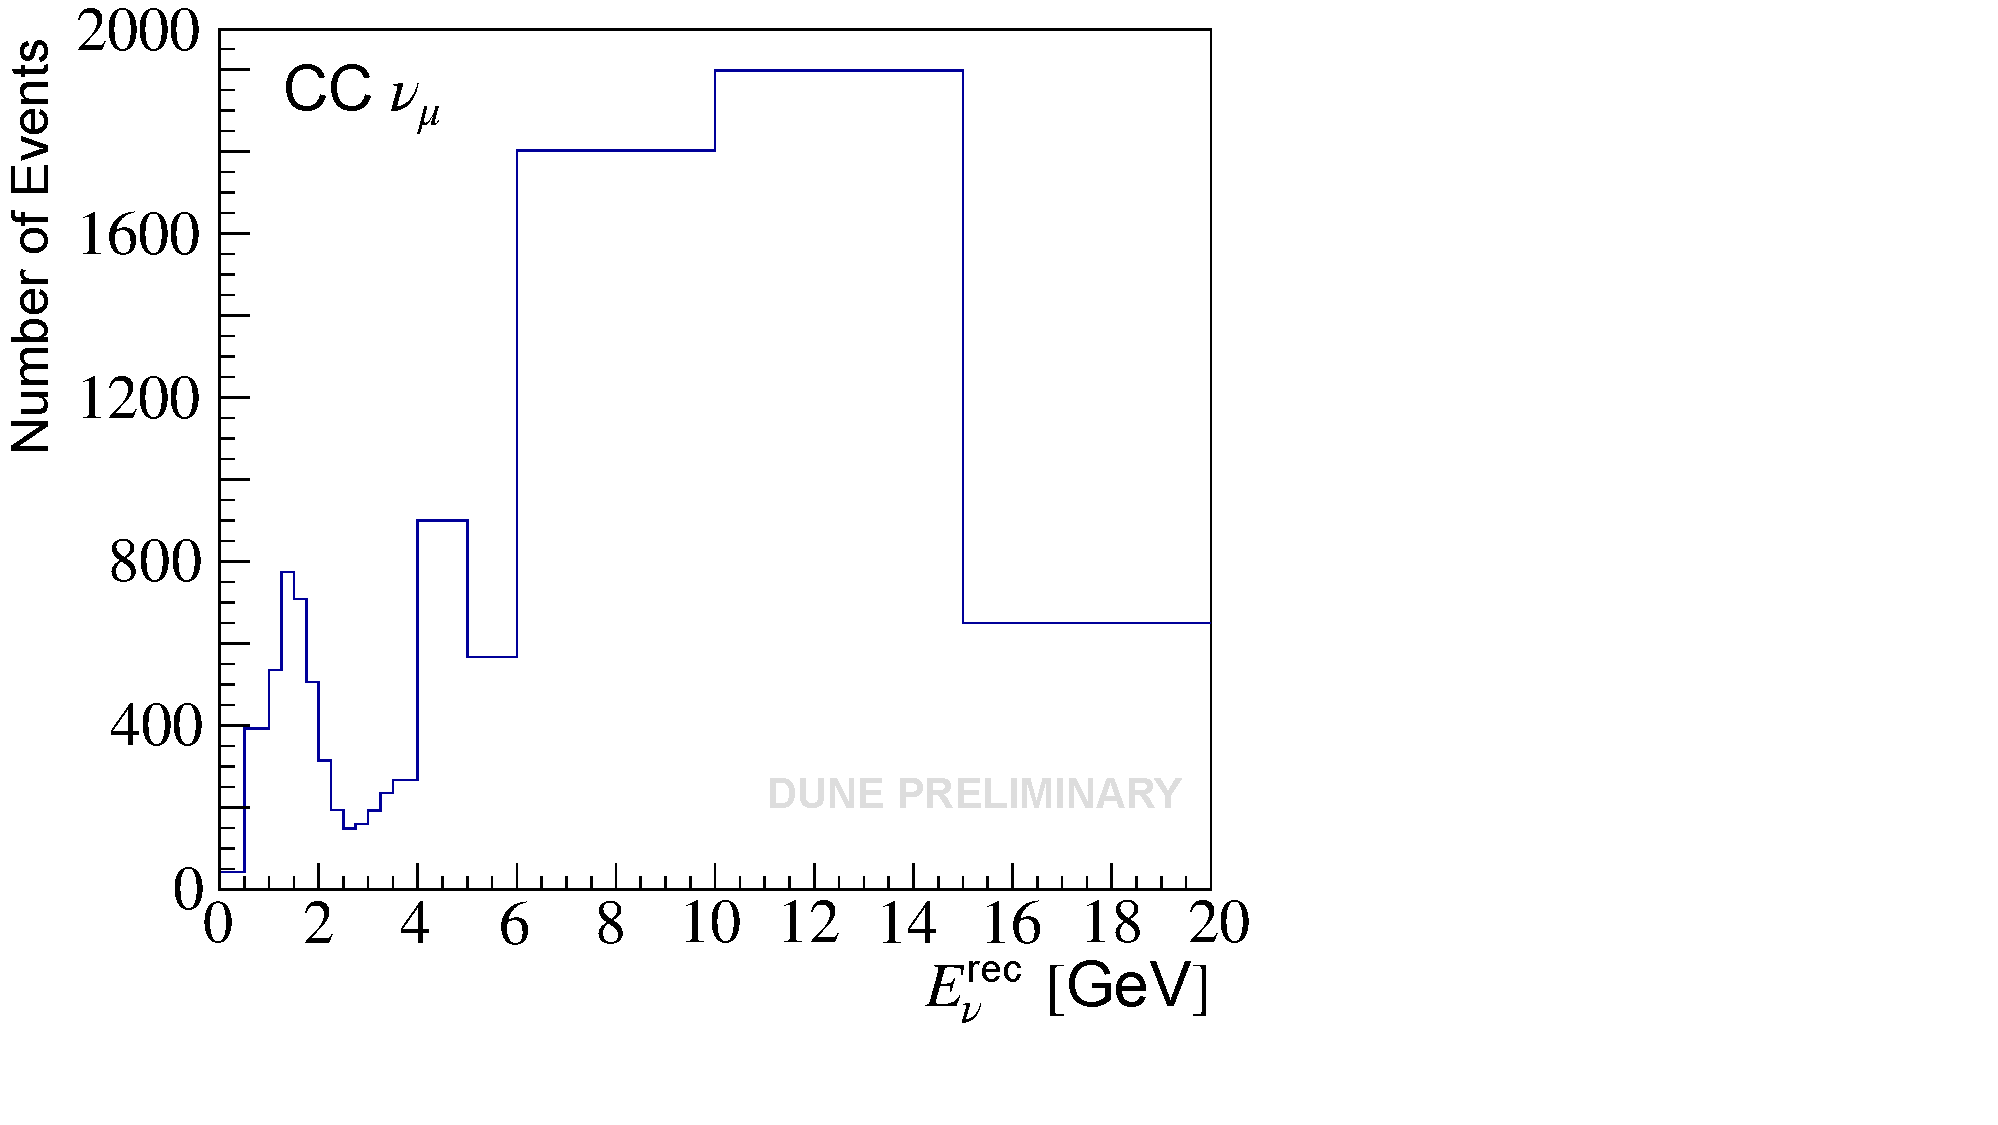
\includegraphics[width=\textwidth]
            {figures/DUNE_EventRate_FHC_CCnumu2.pdf}}}$%{figures/DUNE_EventRate_FHC_CCnumu.pdf}}}$
	\end{minipage}
	\begin{minipage}[b]{.49\textwidth}
		$\vcenter{\hbox{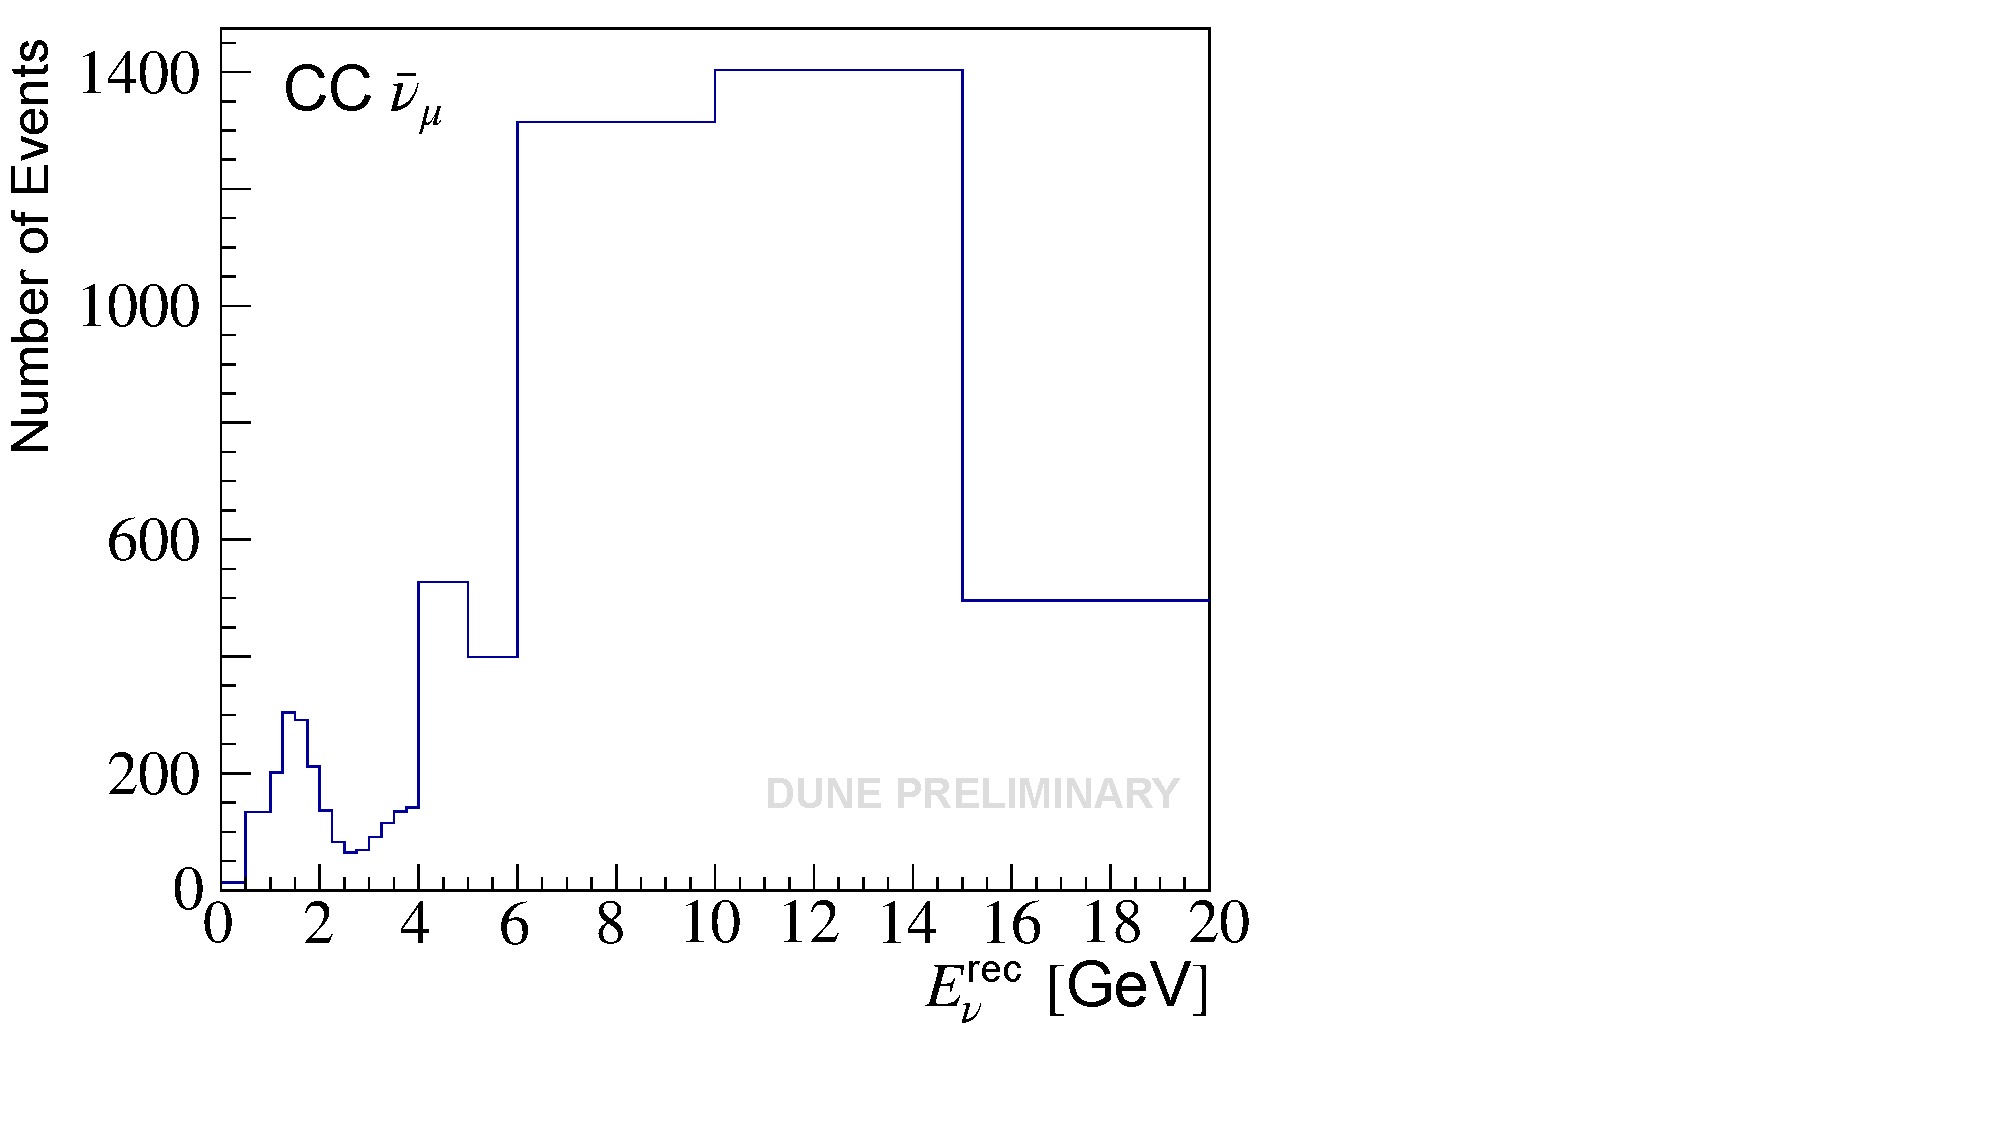
\includegraphics[width=\textwidth]
        {figures/DUNE_EventRate_RHC_CCnumu2.pdf}}}$
        %{figures/DUNE_EventRate_RHC_CCnumu.pdf}}}$
	\end{minipage}
	\vskip\baselineskip
	\begin{minipage}[b]{.49\textwidth}
			$\vcenter{\hbox{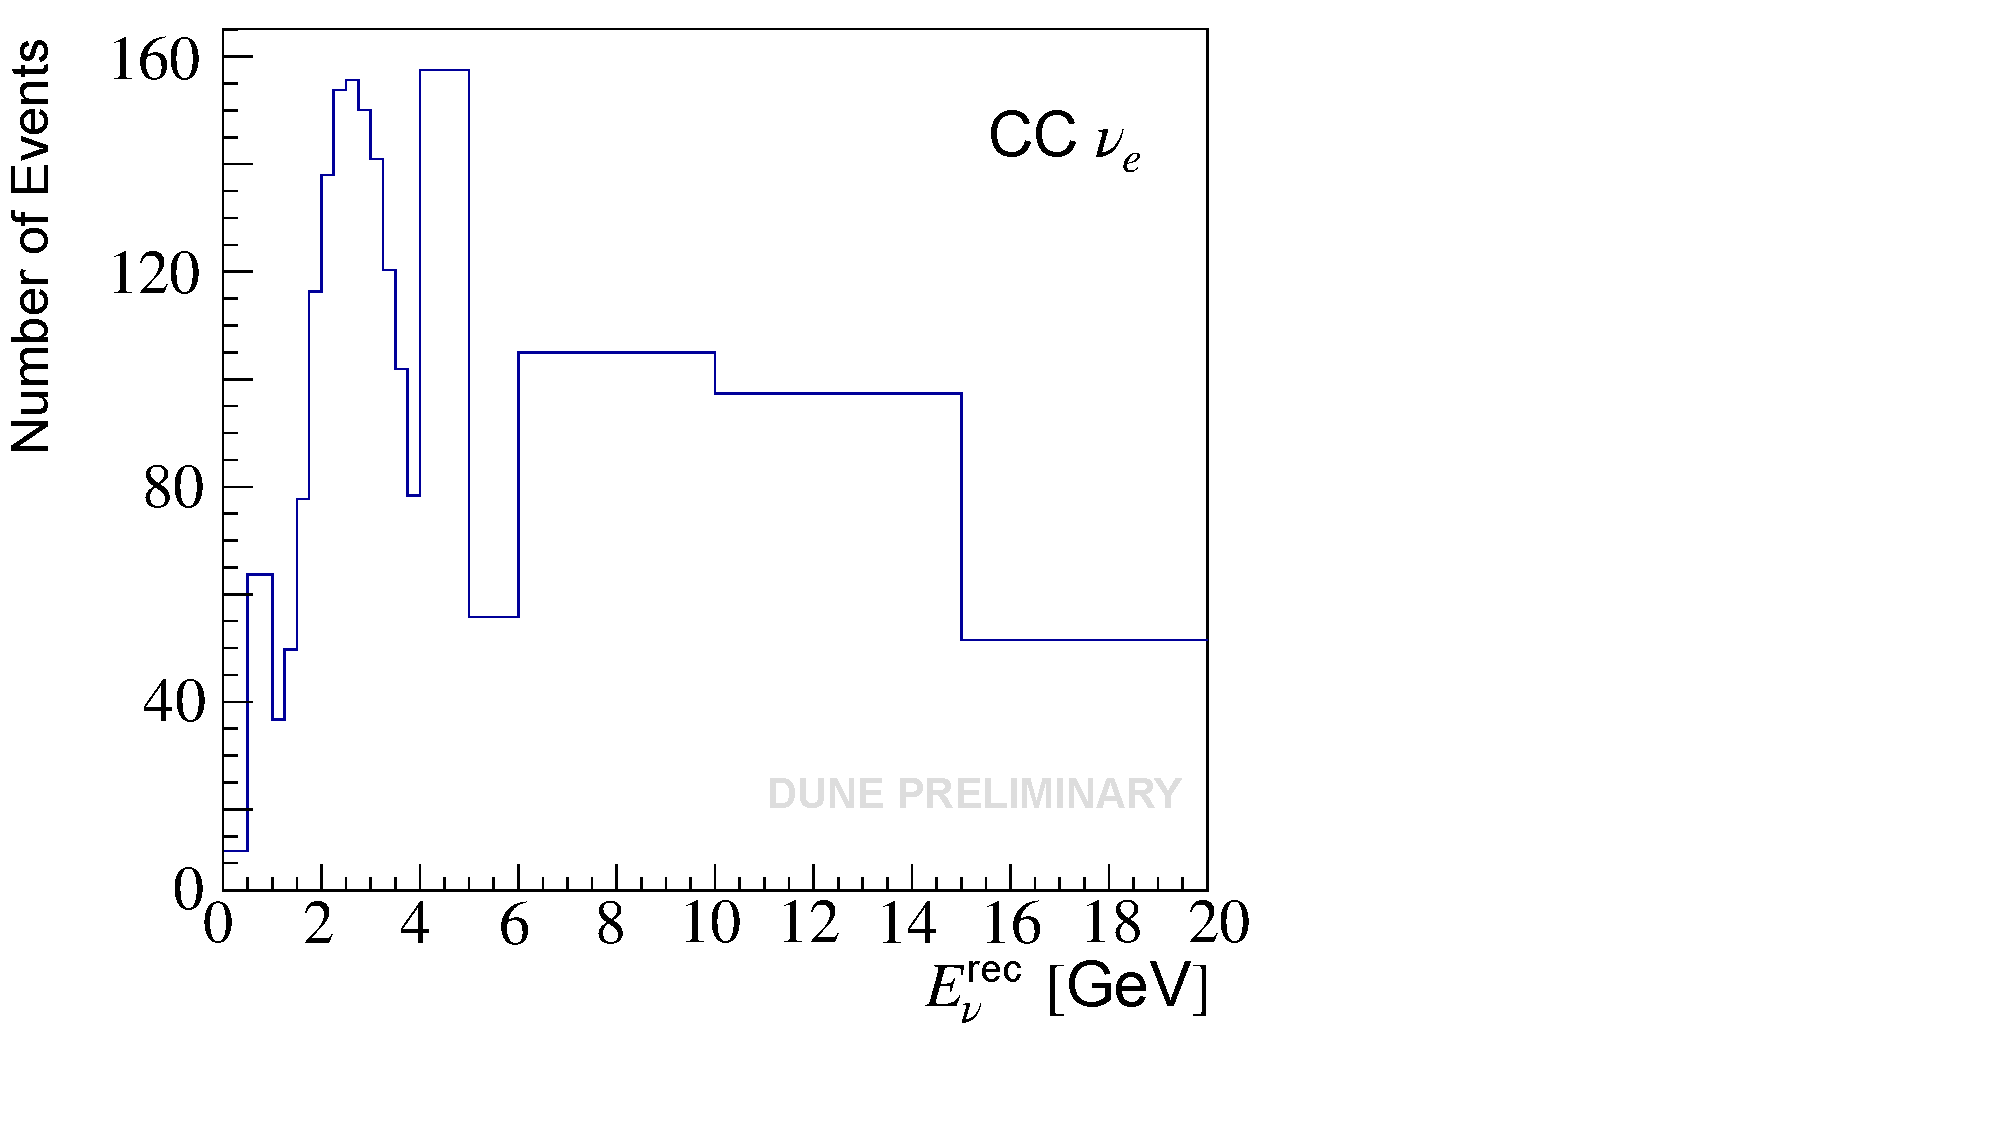
\includegraphics[width=\textwidth]
            {figures/DUNE_EventRate_FHC_CCnue2.pdf}}}$
            %{figures/DUNE_EventRate_FHC_CCnue.pdf}}}$
	\end{minipage}
	\begin{minipage}[b]{.49\textwidth}
		$\vcenter{\hbox{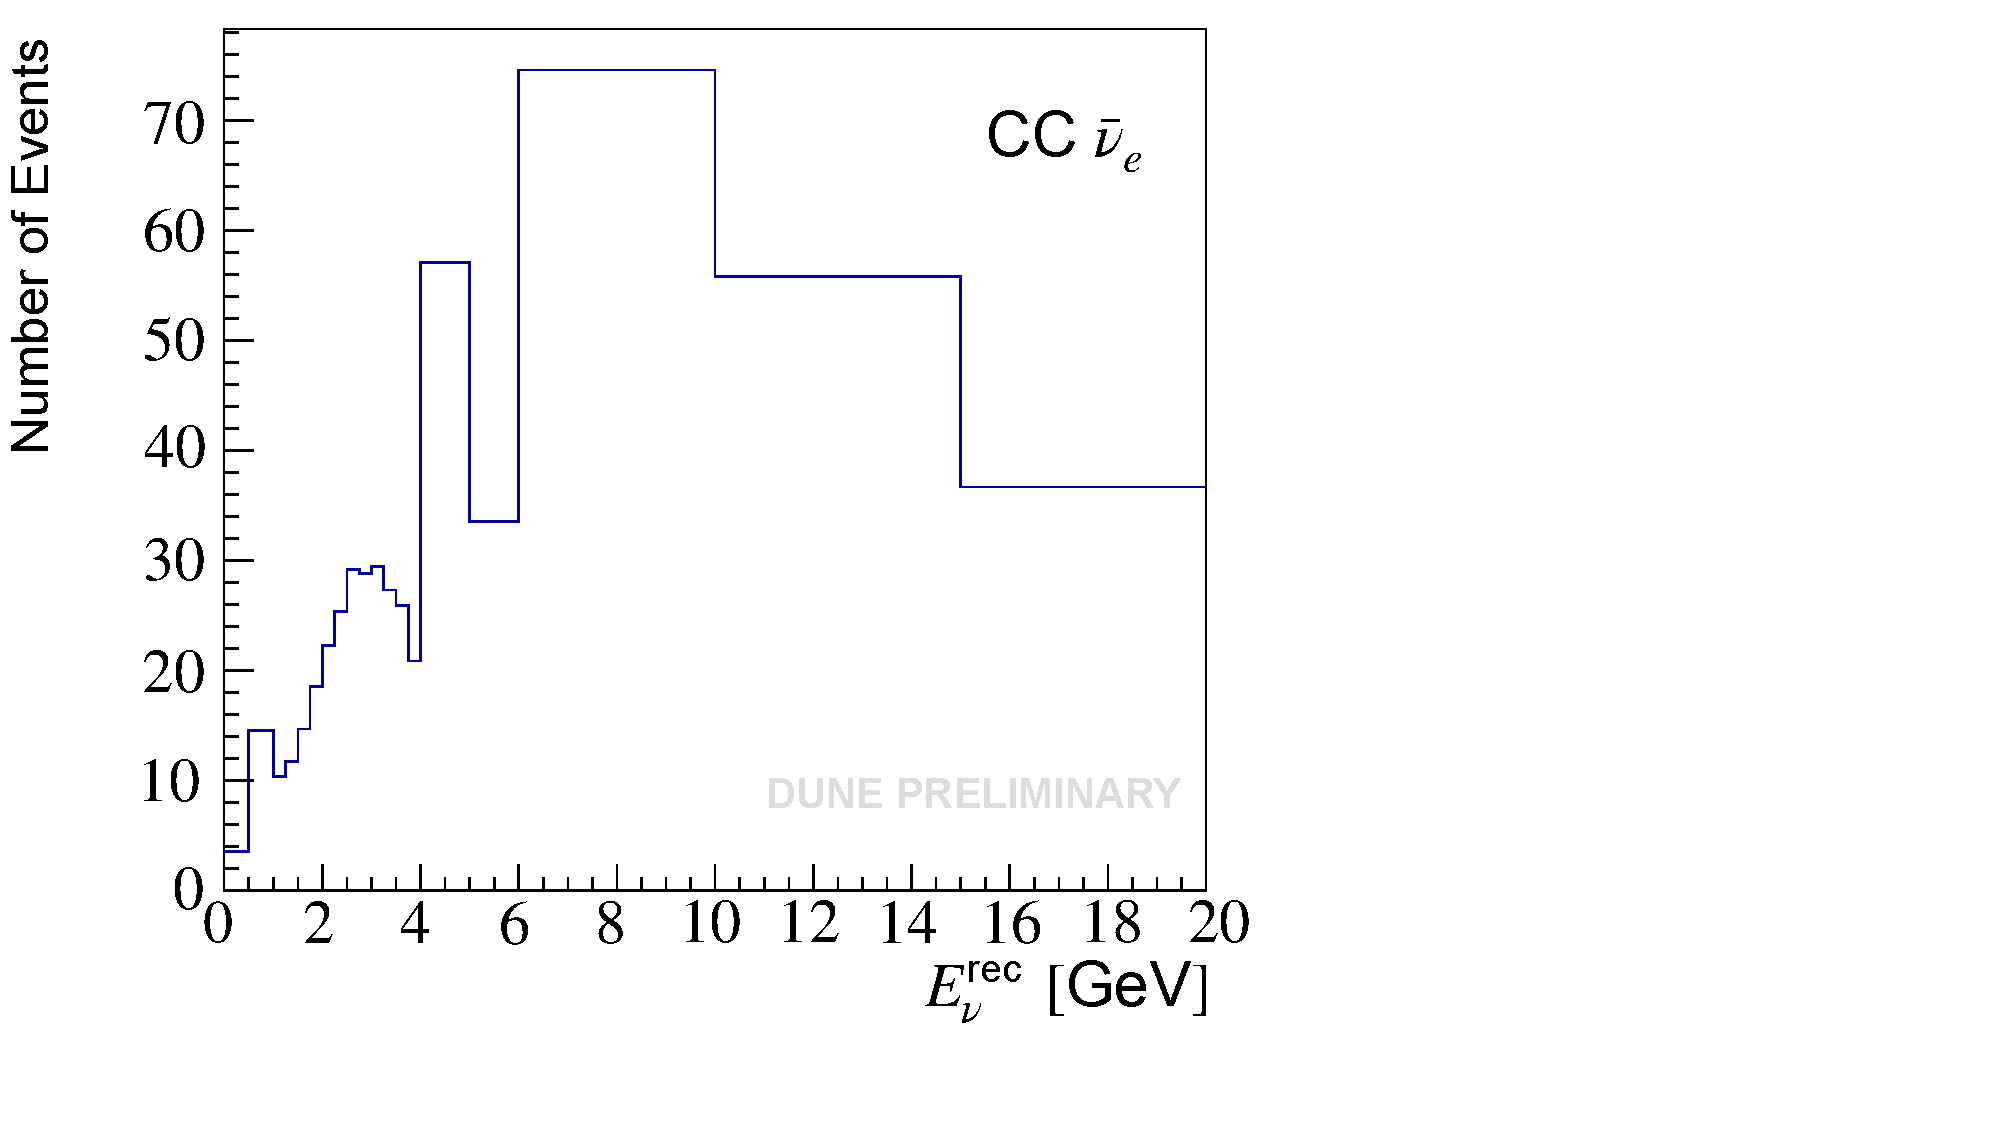
\includegraphics[width=\textwidth]
        {figures/DUNE_EventRate_RHC_CCnue2.pdf}}}$
        %{figures/DUNE_EventRate_RHC_CCnue.pdf}}}$
	\end{minipage}
	\caption{\acrshort{mach3} event spectra predictions at the \acrshort{dune} \acrshort{fd}. The samples are labeled by their interaction topology.}
	\label{fig:event_spectra_dune}
\end{figure}
%
After $\nu_\mu$- and $\nu_e$-interactions are simulated and reconstructed in the \acrshort{dune} \acrshort{fd}, neutrino interactions are classified via a \acrfull{cnn} image recognition and event selection algorithm. An event is selected if it passes flavour classification and fiducial volume cuts. All samples are then binned in reconstructed neutrino energy $E_\nu^\text{rec}$ \cite{DUNE:2020ypp}.% {\color{red} What do I cite here (as this is described in a DUNE tech-note)?}

\subsection{\texorpdfstring{\acrshort{t2k}}{TEXT} \texorpdfstring{\acrshort{mc}}{TEXT} Samples and Event Selection} \label{sec:t2k_selection}
%
%\ohead{\ref{sec:t2k_selection} \ \acrshort{t2k} \acrshort{mc} Samples and Event Selection}
%
The available reconsructed \acrshort{mc} data samples in \acrshort{t2k} are the \acrfull{cc} muon neutrino and muon anti-neutrino pionless ($\nu_\mu$\acrshort{cc}$0\pi$ and $\bar{\nu}_\mu$\acrshort{cc}$0\pi$), \acrlong{cc} electron neutrino and electron anti-neutrino pionless ($\nu_e$\acrshort{cc}$0\pi$ and $\bar{\nu}_e$\acrshort{cc}$0\pi$) and the %hybrid\footnote{Here, 'hybrid samples' refer to data-driven \acrshort{mc} samples that are constructed by modifying real atmospheric neutrino data events in \acrshort{sk} to resemble certain types of signal events, in this case, $\nu_\mu$ \acrshort{cc}$1\pi^+$ interactions.}
\acrlong{cc} muon- and electron-neutrino with one positively-charged pion ($\nu_\mu$\acrshort{cc}$1\pi^+$ and $\nu_e$\acrshort{cc}$1\pi^+$) samples, as shown in \Cref{fig:event_spectra_t2k}. 
%
\begin{figure}[H]
	\begin{minipage}[b]{.49\textwidth}
			$\vcenter{\hbox{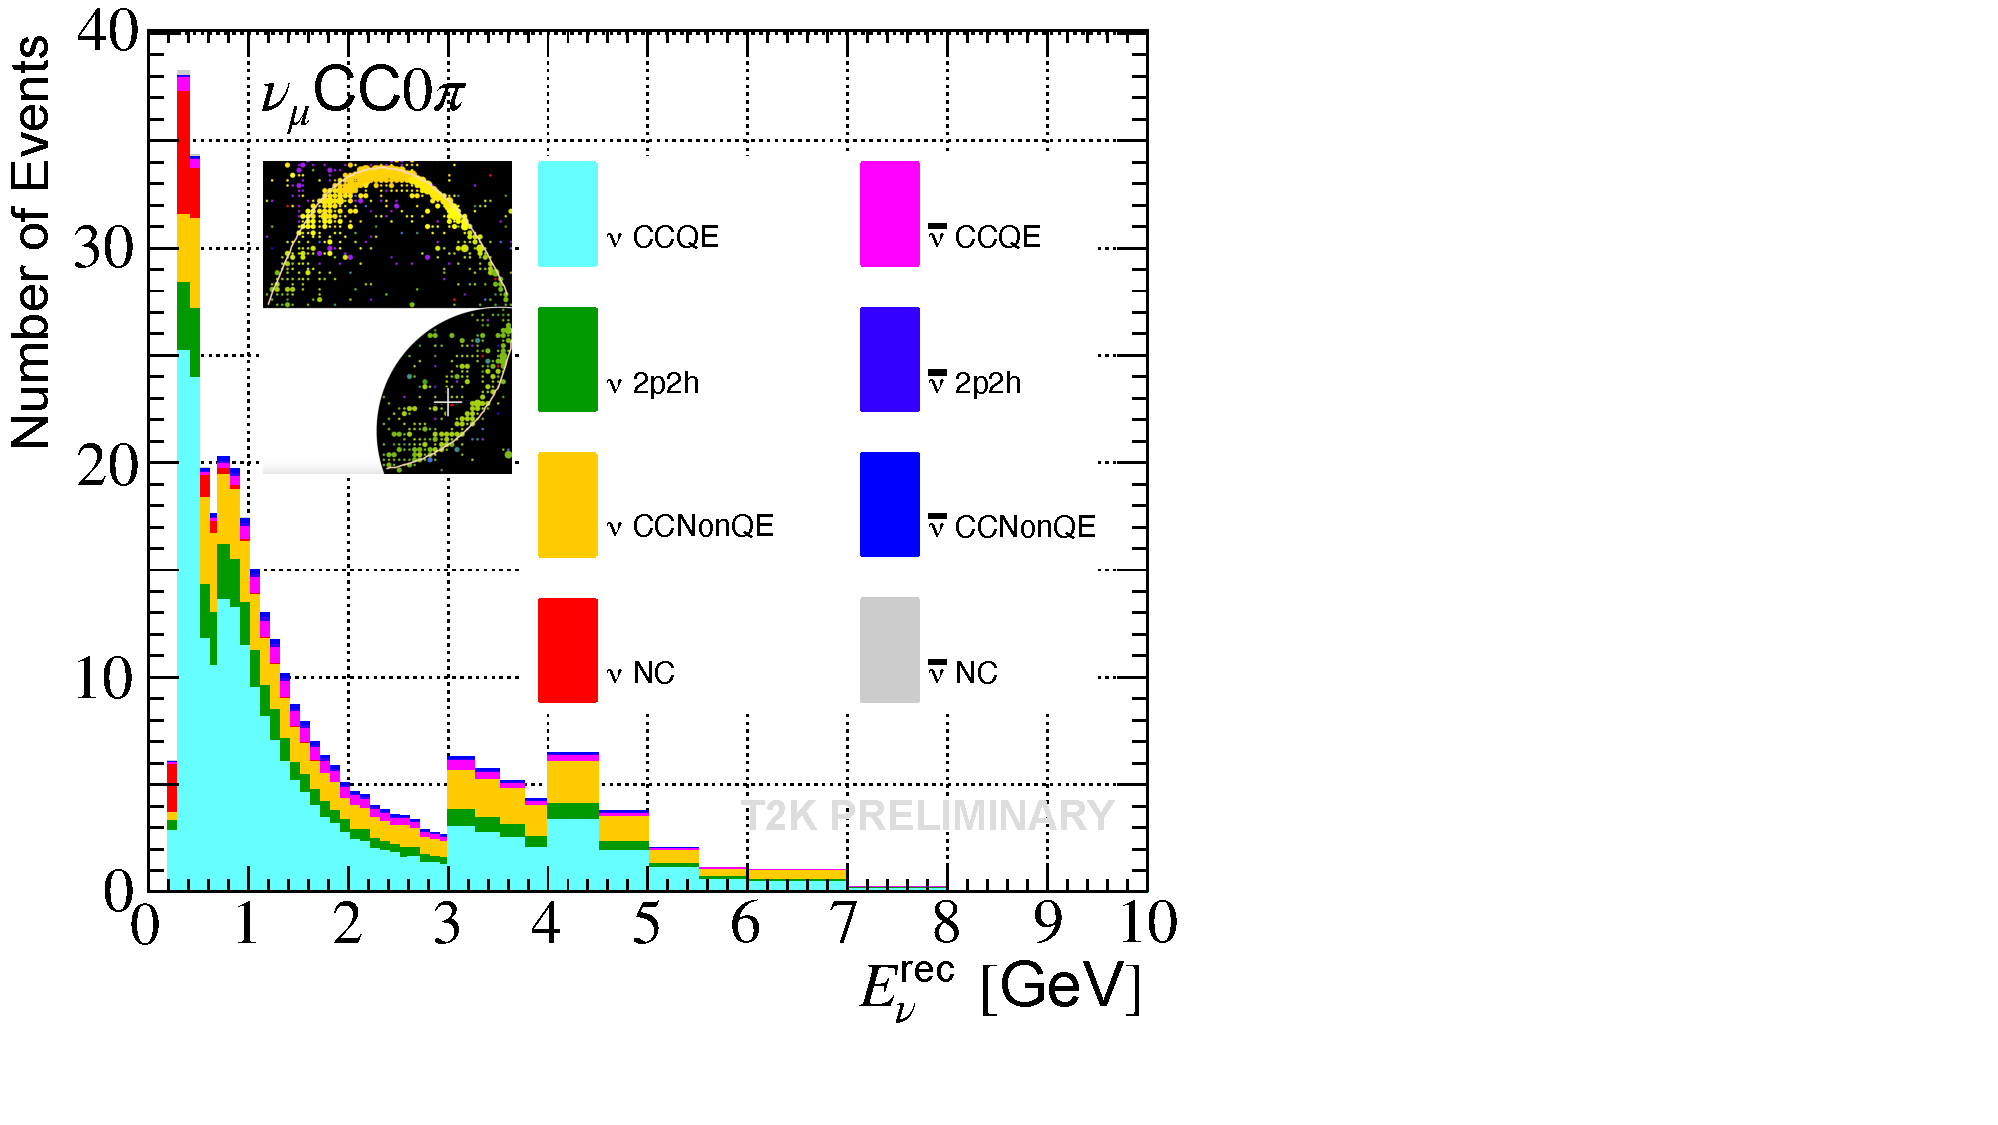
\includegraphics[width=\textwidth]
            {figures/T2K_FHC1Rmu_2024_all2}}}%{figures/T2K_FHC1Rmu_2024_all}}}%{figures/T2K_FHC1Rmu_2024_logo}}}%{figures/T2K_FHC1Rmu_2024}}}%{figures/test_t2k_outputfile_SKEventRates_Plots_ErecModeOscChanBreakdown_FHC_1Rmu_2024.pdf}}}
            $
	\end{minipage}
	\begin{minipage}[b]{.49\textwidth}
		$\vcenter{\hbox{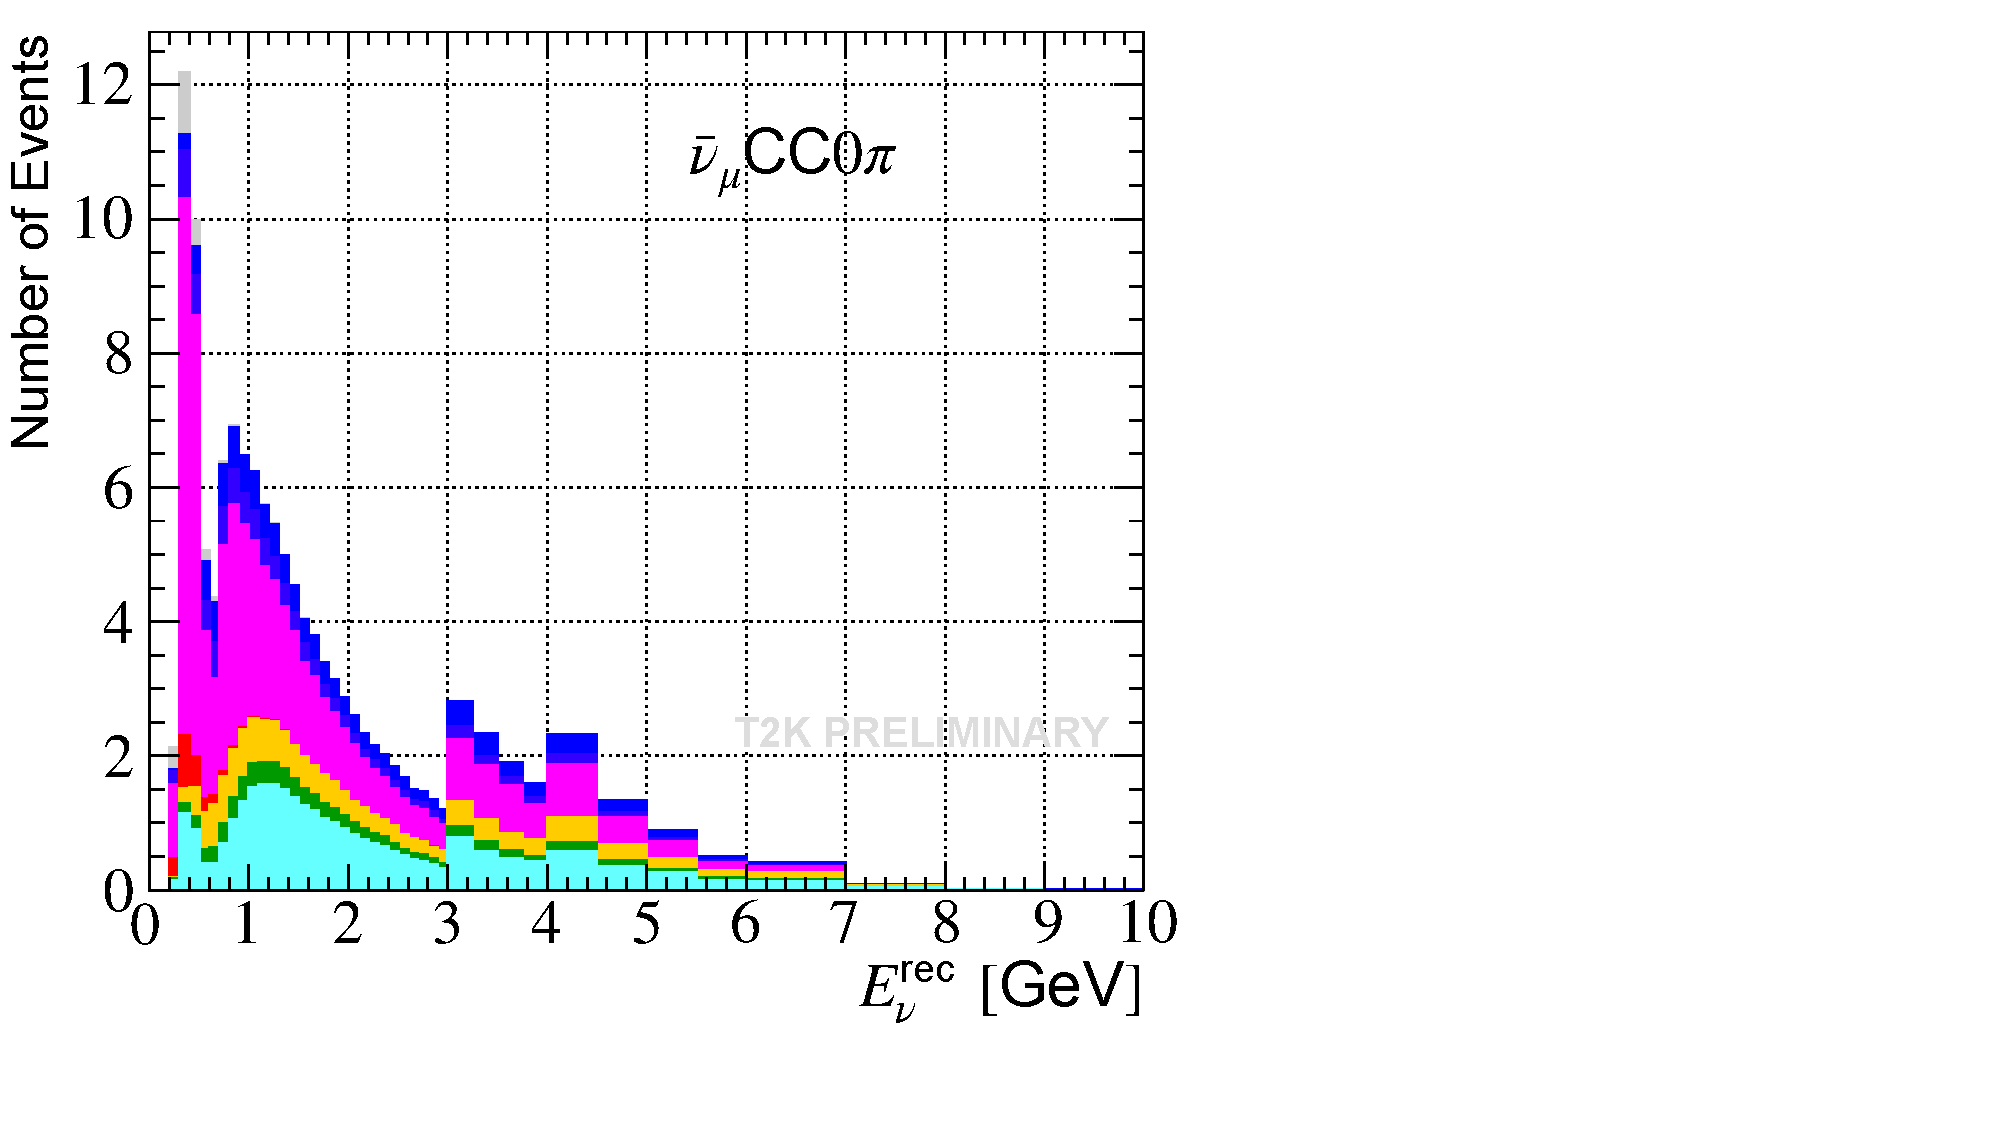
\includegraphics[width=\textwidth]
        {figures/T2K_RHC1Rmu_2024_noLogo_noLegend2.pdf}}}$
        %{figures/T2K_RHC1Rmu_2024_noLogo_noLegend.pdf}}}$
        %{figures/T2K_RHC1Rmu_2024_noLegend.pdf}}}$
        %{figures/T2K_RHC1Rmu_2024.pdf}}}$
	\end{minipage}
	\vskip\baselineskip
	\begin{minipage}[b]{.49\textwidth}
			$\vcenter{\hbox{\includegraphics[width=\textwidth]%
            {figures/T2K_FHCnumuCC1pi_20242.pdf}}}$
            %{figures/T2K_FHCnumuCC1pi_2024.pdf}}}$
	\end{minipage}
	\begin{minipage}[b]{.49\textwidth}
		$\vcenter{\hbox{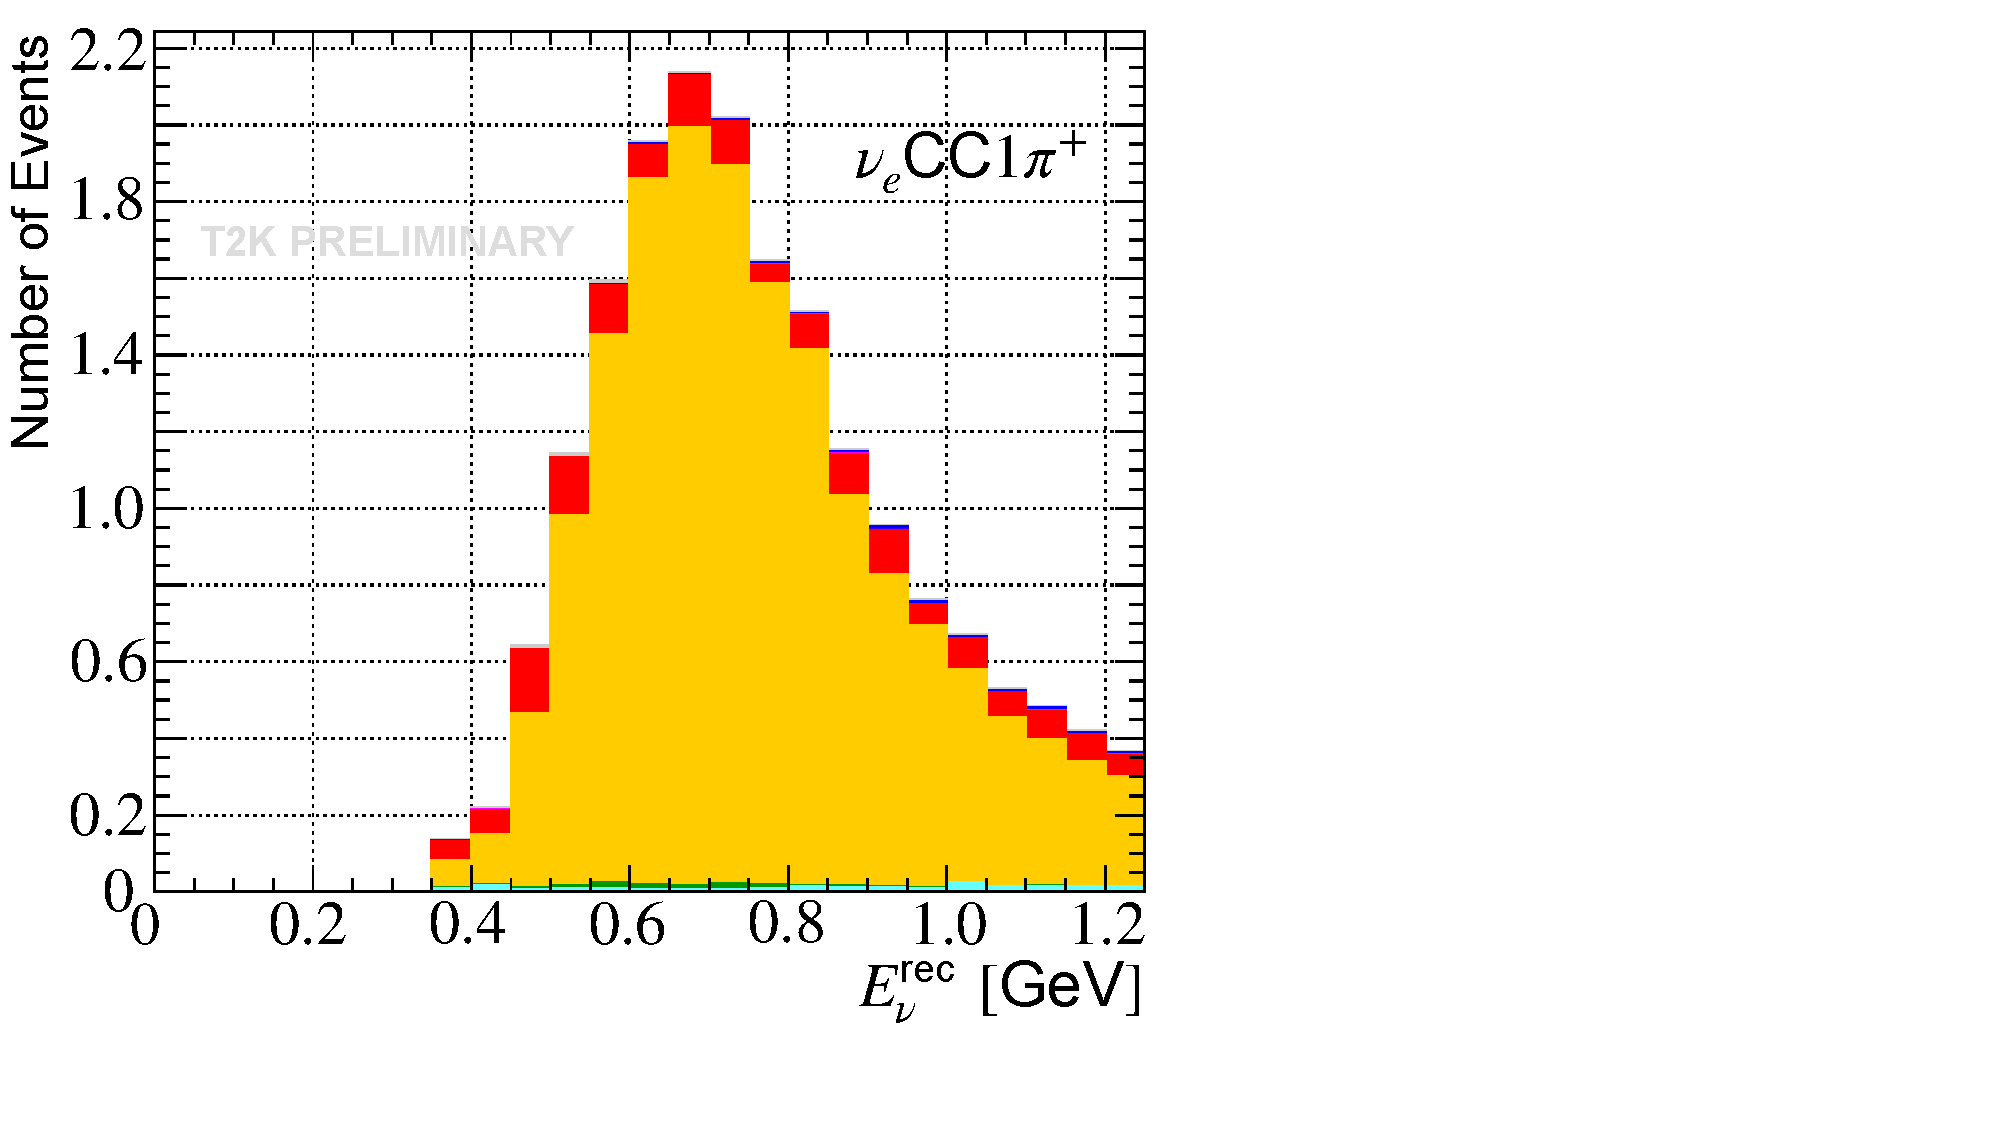
\includegraphics[width=\textwidth]
        {figures/T2K_FHCnueCC1pi_20242.pdf}}}$
        %{figures/T2K_FHCnueCC1pi_2024.pdf}}}$
	\end{minipage}
	\vskip\baselineskip
	\begin{minipage}[b]{.49\textwidth}
		$\vcenter{\hbox{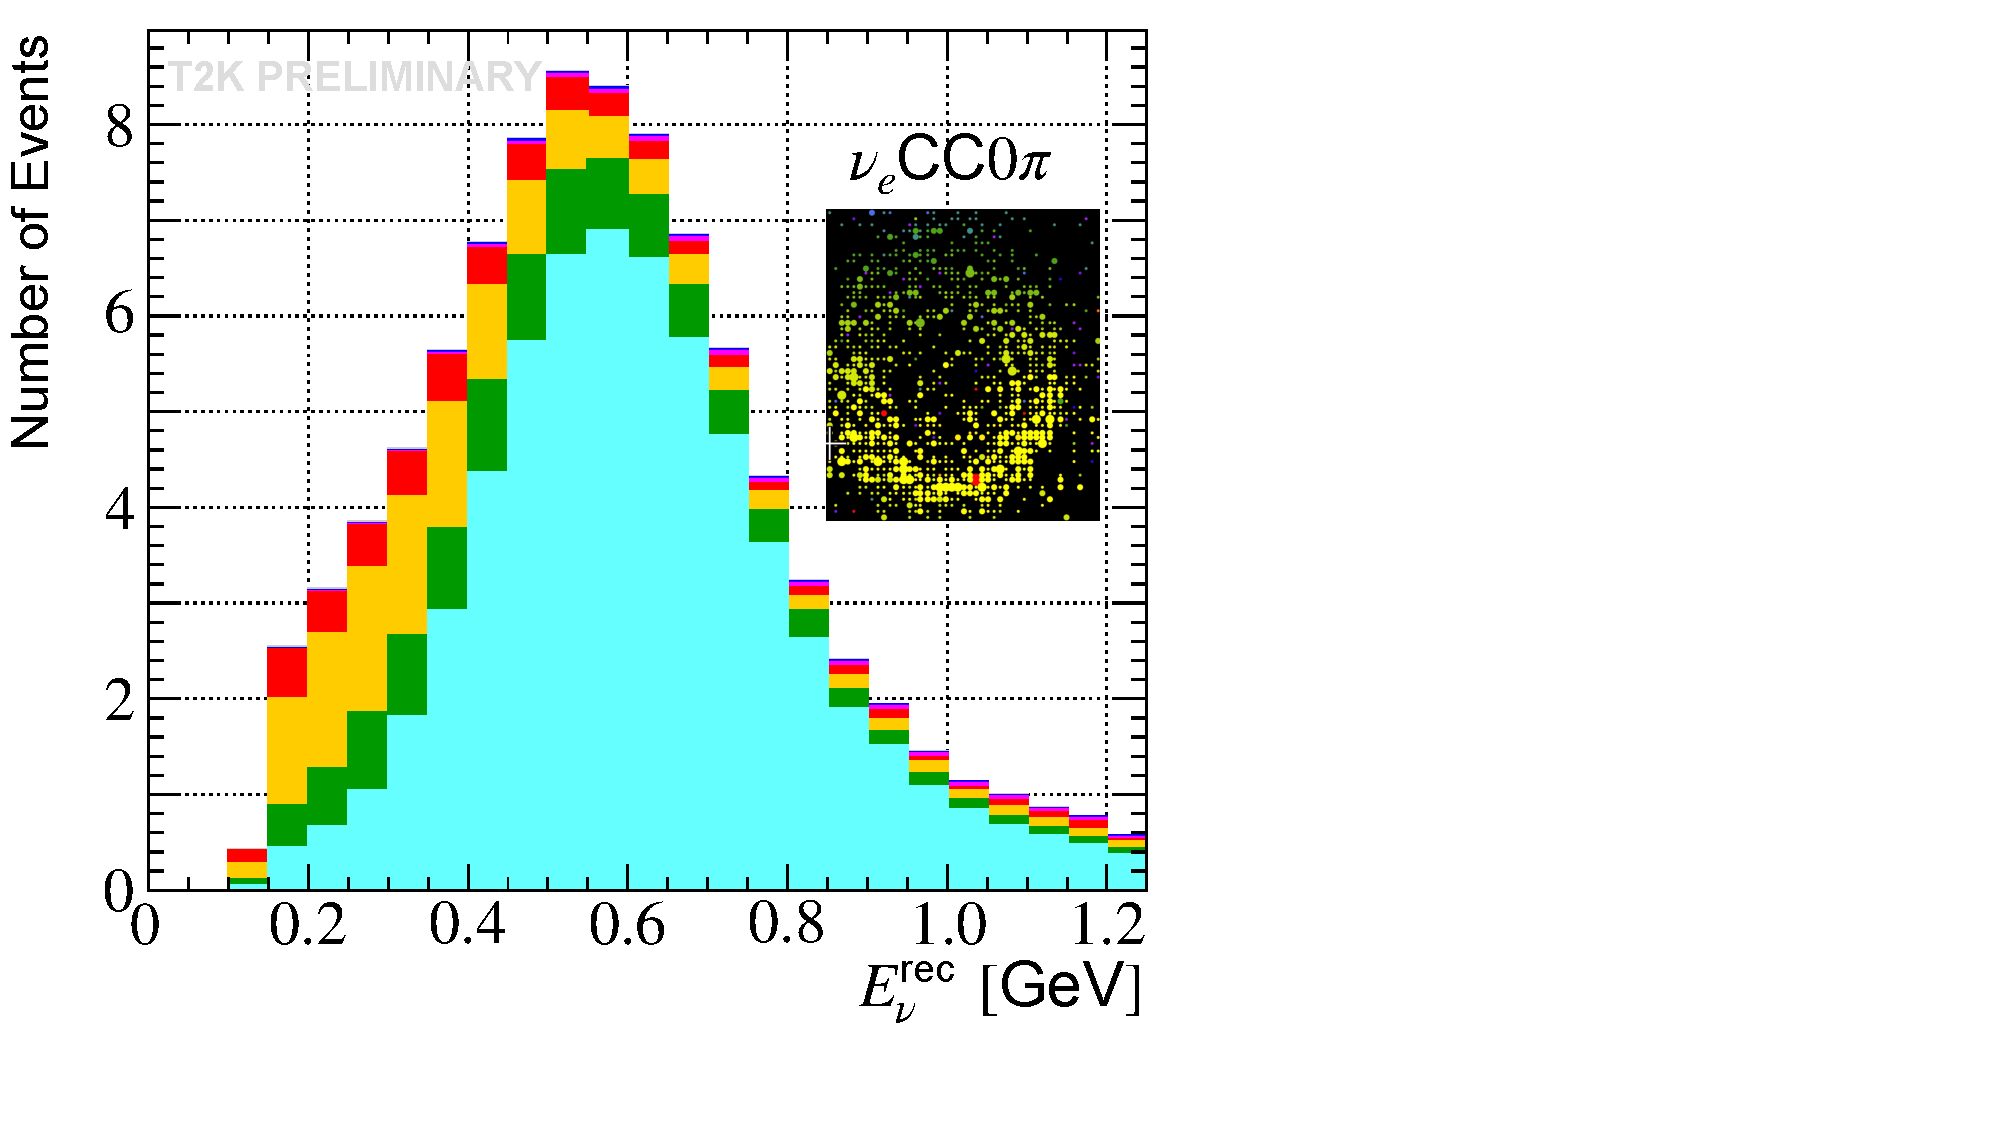
\includegraphics[width=\textwidth]
        {figures/T2K_FHC1Re_2024_all2.pdf}}}%
        %{figures/T2K_FHC1Re_2024_all.pdf}}}%{figures/T2K_FHC1Re_2024.pdf}}}%
        ]$
	\end{minipage}
	\begin{minipage}[b]{.49\textwidth}
		$\vcenter{\hbox{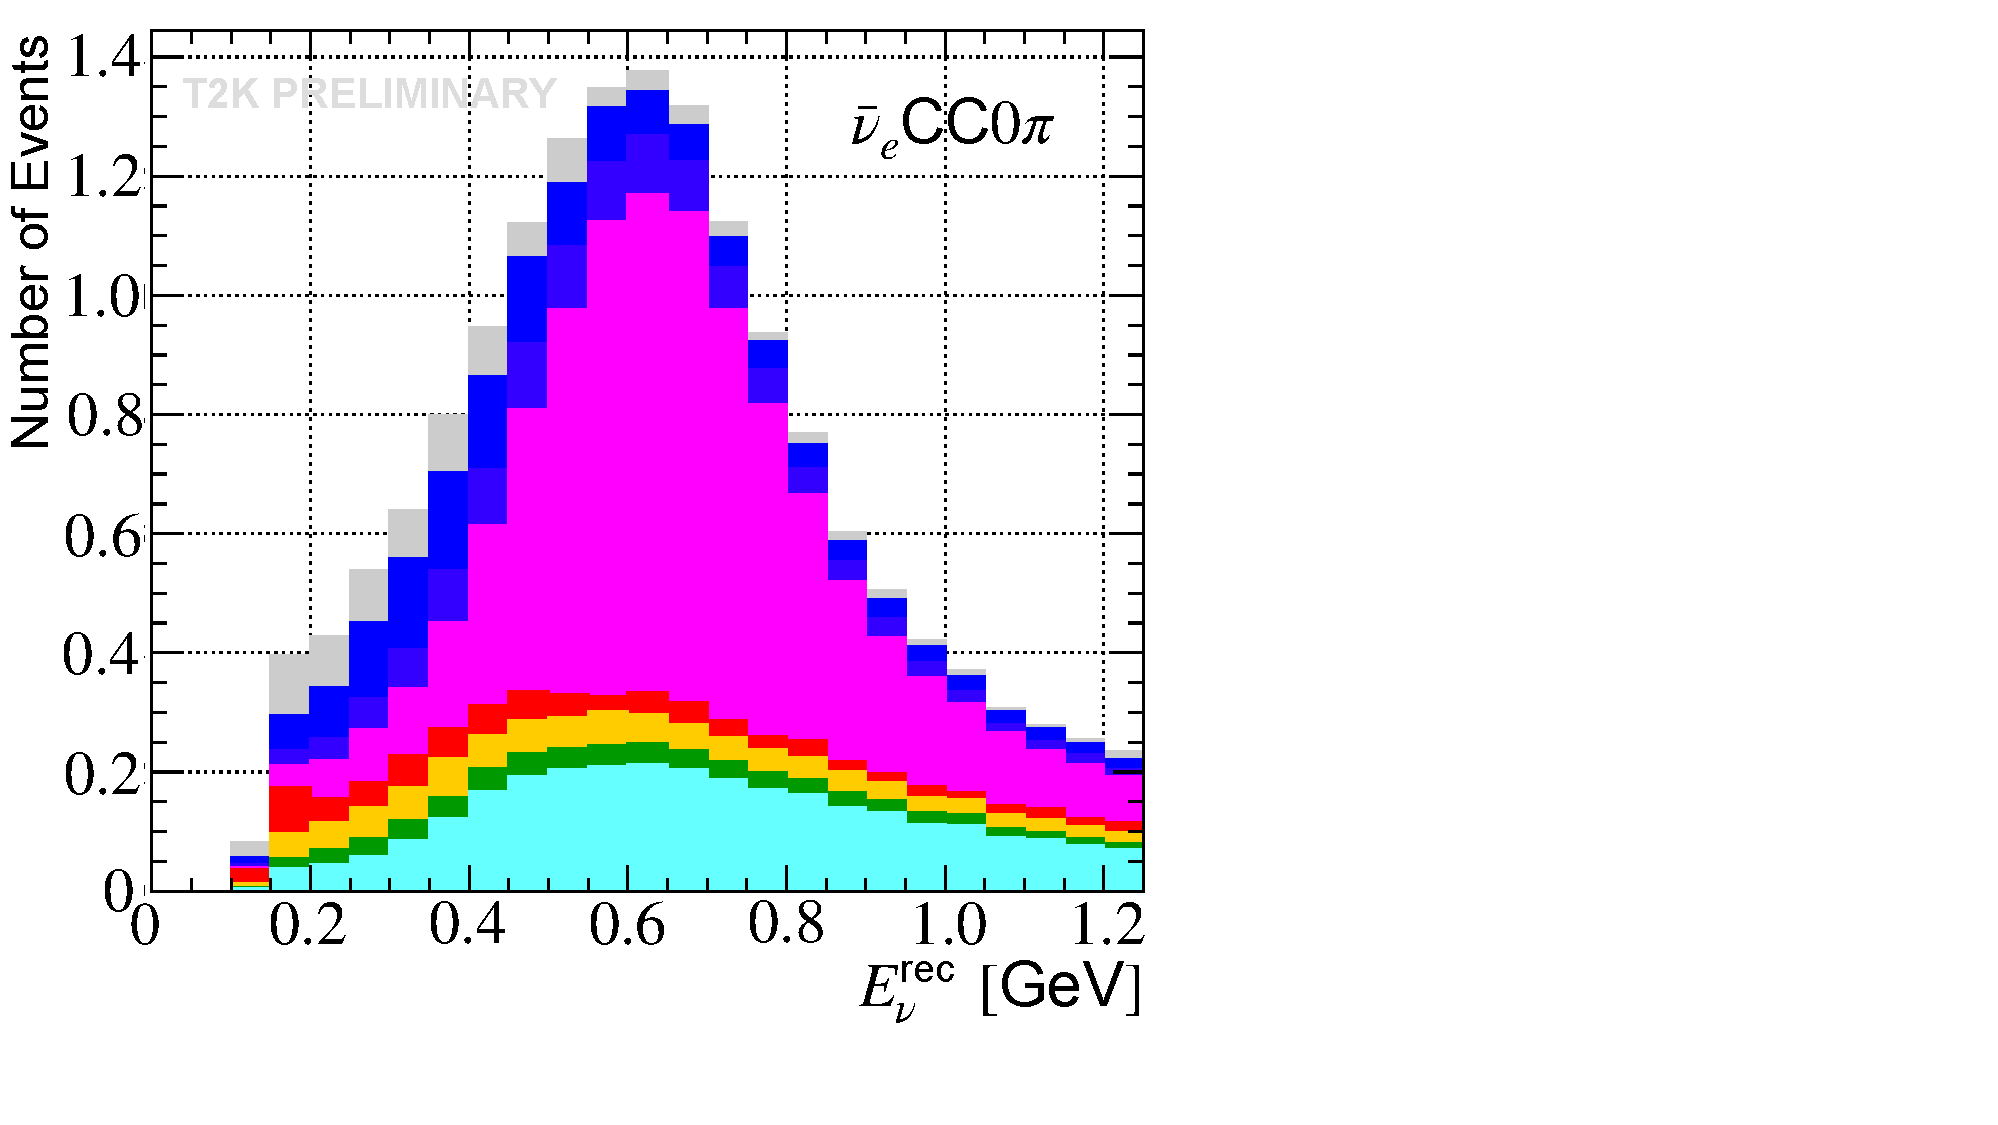
\includegraphics[width=\textwidth]
        {figures/T2K_RHC1Re_2024_noLogo2.pdf}}}$
        %{figures/T2K_RHC1Re_2024_noLogo.pdf}}}$
        %{figures/T2K_RHC1Re_2024.pdf}}}$
	\end{minipage}
	\caption{\acrshort{mach3} event spectra predictions broken down by interaction modes at the Super-Kamiokande (\acrshort{t2k} \acrshort{fd}). The samples are labeled by their interaction topology. Write out interaction modes acrshort{ccqe}, acrshort cc res etc..}
	\label{fig:event_spectra_t2k}
\end{figure}
%
The \acrshort{t2k} \acrshort{fd} called Super-Kamiokande is a Cherenkov detector filled with Gadolinium-doped water. The event selection is performed by identifying Cherenkov rings produced by muons or electrons originating from $\nu_\mu$ or $\nu_e$-like interactions inside Super-Kamiokande. A \acrshort{fhc} $\nu_\mu$ \acrshort{cc}$1\pi^+$ event is identified by a primary muon ring which has a decay electron and also has an additional decay electron from the pion decay. The \acrshort{fhc} $\nu_e$ \acrshort{cc}$1\pi^+$ event looks for an associated primary electron ring with an associated decay electron from the invisible pion decay. %{\color{red} More details on samples?}

After $\nu_\mu$- and $\nu_e$-interactions are simulated and reconstructed in the \acrshort{t2k} \acrshort{fd}, there is a matching of kinematics between a T$2$K 
\acrshort{mc} and an \acrshort{sk} atmospheric muon event and generating \acrshort{mc} charged pion rings. Neutrino interactions are then classified via a maximum likelihood fitter called FitQUN. An event is selected if it passes flavour classification and fiducial volume cuts. Most \acrshort{t2k} samples are then binned in both reconstructed neutrino energy $E_\nu^\text{rec}$ and lepton direction \cite{t2k-tech-342_numu,t2k-tech-389_nue}.%{\color{red} What do I cite here (as this is described in a T2K tech-notes)?}

\subsection{Simulations and Systematic Uncertainties} \label{sec:sim_and_uncertainties}
%
%\ohead{\rightmark}
%
%In the results presented in \Cref{sec:results}, s
Several models for the simulation of flux, detector response and cross-section predictions with respective systematic uncertainties that differ between \acrshort{dune} and \acrshort{t2k} have been taken into account in \acrshort{mach3}. The systematic uncertainties in the neutrino flux are predominantly due to correlated uncertainties in the hadron production and beam production models. Uncertainties in the \acrshort{fd} concern the modeling of the detector geometry and properties as well as in the event reconstruction and how this affects the reconstructed neutrino energy. Cross-section systematic uncertainties are categorised according to nuclear effects and the type of the neutrino interaction. The largest fraction of all systematic uncertainties can be attributed to cross-section uncertainties (see \Cref{tab:uncertainties}).
%
\begin{table}[H]
    \centering
    \caption[]{Uncertainties [$\%$] on the \acrshort{dune} (left) and \acrshort{t2k} (right) \acrlong{fd} for each sample, grouped by uncertainty category. Data taken from \cite{dune-OA,t2k-OA}.}
    \label{tab:uncertainties}
    \begin{minipage}{0.44\textwidth}
        \centering
        \begin{tabular}{|l||c|c|c|c|}
            \hline
            \textbf{\acrshort{dune}} & $\boldsymbol{\nu_\mu}$ & $\bar{\boldsymbol{\nu}_\mu}$ & $\boldsymbol{\nu_e}$ & $\boldsymbol{\bar{\nu}_e}$ \\ \hline \hline
            \textbf{Flux} & $7.3$ & $7.5$ & $7.3$ & $7.3$ \\ \hline
            \textbf{Detector} & $2.3$ & $2.7$ & $1.7$ & $2.0$ \\ \hline
            \textbf{Cross-Sec.} & $9.3$ & $7.8$ & $9.2$ & $7.9$ \\ \hline \hline
            \textbf{Total Syst.} & $11.9$ & $11.1$ & $11.7$ & $10.7$ \\ \hline \hline
            \textbf{Statistical} & $1.0$ & $1.5$ & $2.2$ & $4.4$ \\
            \hline \hline
        \end{tabular}
    \end{minipage}
    \hfill
    \begin{minipage}[t]{0.55\textwidth}
        \vspace{-18.5mm}
        %\centering
        \begin{tabular}{|l||c|c|c|c|c|c|}
            \hline
            \textbf{\acrshort{t2k}} & $\boldsymbol{\nu_\mu}$ & $\bar{\boldsymbol{\nu}_\mu}$ & $\boldsymbol{\nu_\mu}1\pi^+$ & $\boldsymbol{\nu_e}$ & $\boldsymbol{\bar{\nu}_e}$ & $\boldsymbol{\nu_e}1\pi^+$ \\ \hline \hline
             & 2.72 & 2.80 & 2.79 & 2.75 & 2.88 & 2.81 \\ \hline
             & 1.43 & 3.34 & 0.10 & 2.74 & 5.03 & 4.40 \\ \hline
             & 3.45 & 4.42 & 3.21 & 4.44 & 4.92 & 4.69 \\ \hline \hline
             & 2.6 & 4.52 & 2.46 & 4.54 & 6.59 & 6.06 \\ \hline \hline
        \end{tabular}
    \end{minipage}
\end{table}
%

\subsection{Code Implementation} \label{sec:code_implementation}
%{\color{red} Show CUDAProb3 vs NuSQUIDS validation plots here? Show nu and anti-nu oscillation plots somewhere in this document besides fig. 3?}
\acrfull{mach3} is a Bayesian \acrfull{mcmc} fitter for performing oscillation analyses in \acrshort{dune}, T$2$K and other experiments. It is used within standard \acrshort{dune} and T$2$K oscillation analyses and uses standard sample selections in both experiments. Recent developments have allowed the usage of various neutrino oscillation engines that are implemented into the neutrino oscillation probability calculation interface \href{https://github.com/dbarrow257/NuOscillator.git}{NuOscillator}. The NuOscillator code is integrated into and utilised by the \acrshort{mach3} framework. Currently the two neutrino oscillation engines \href{https://zenodo.org/records/14741956}{OscProb} and \href{https://github.com/larsb-p/nuSQuIDS/tree/master/examples}{NuSQuIDS} \cite{Arguelles:2021twb}, provide several implemented \acrshort{bsm} models. This analysis uses the \acrshort{nusquids} code that we recently added to NuOscillator as a new neutrino oscillation calculator engine.
%
    \begin{figure}[hbt]
	\centering
	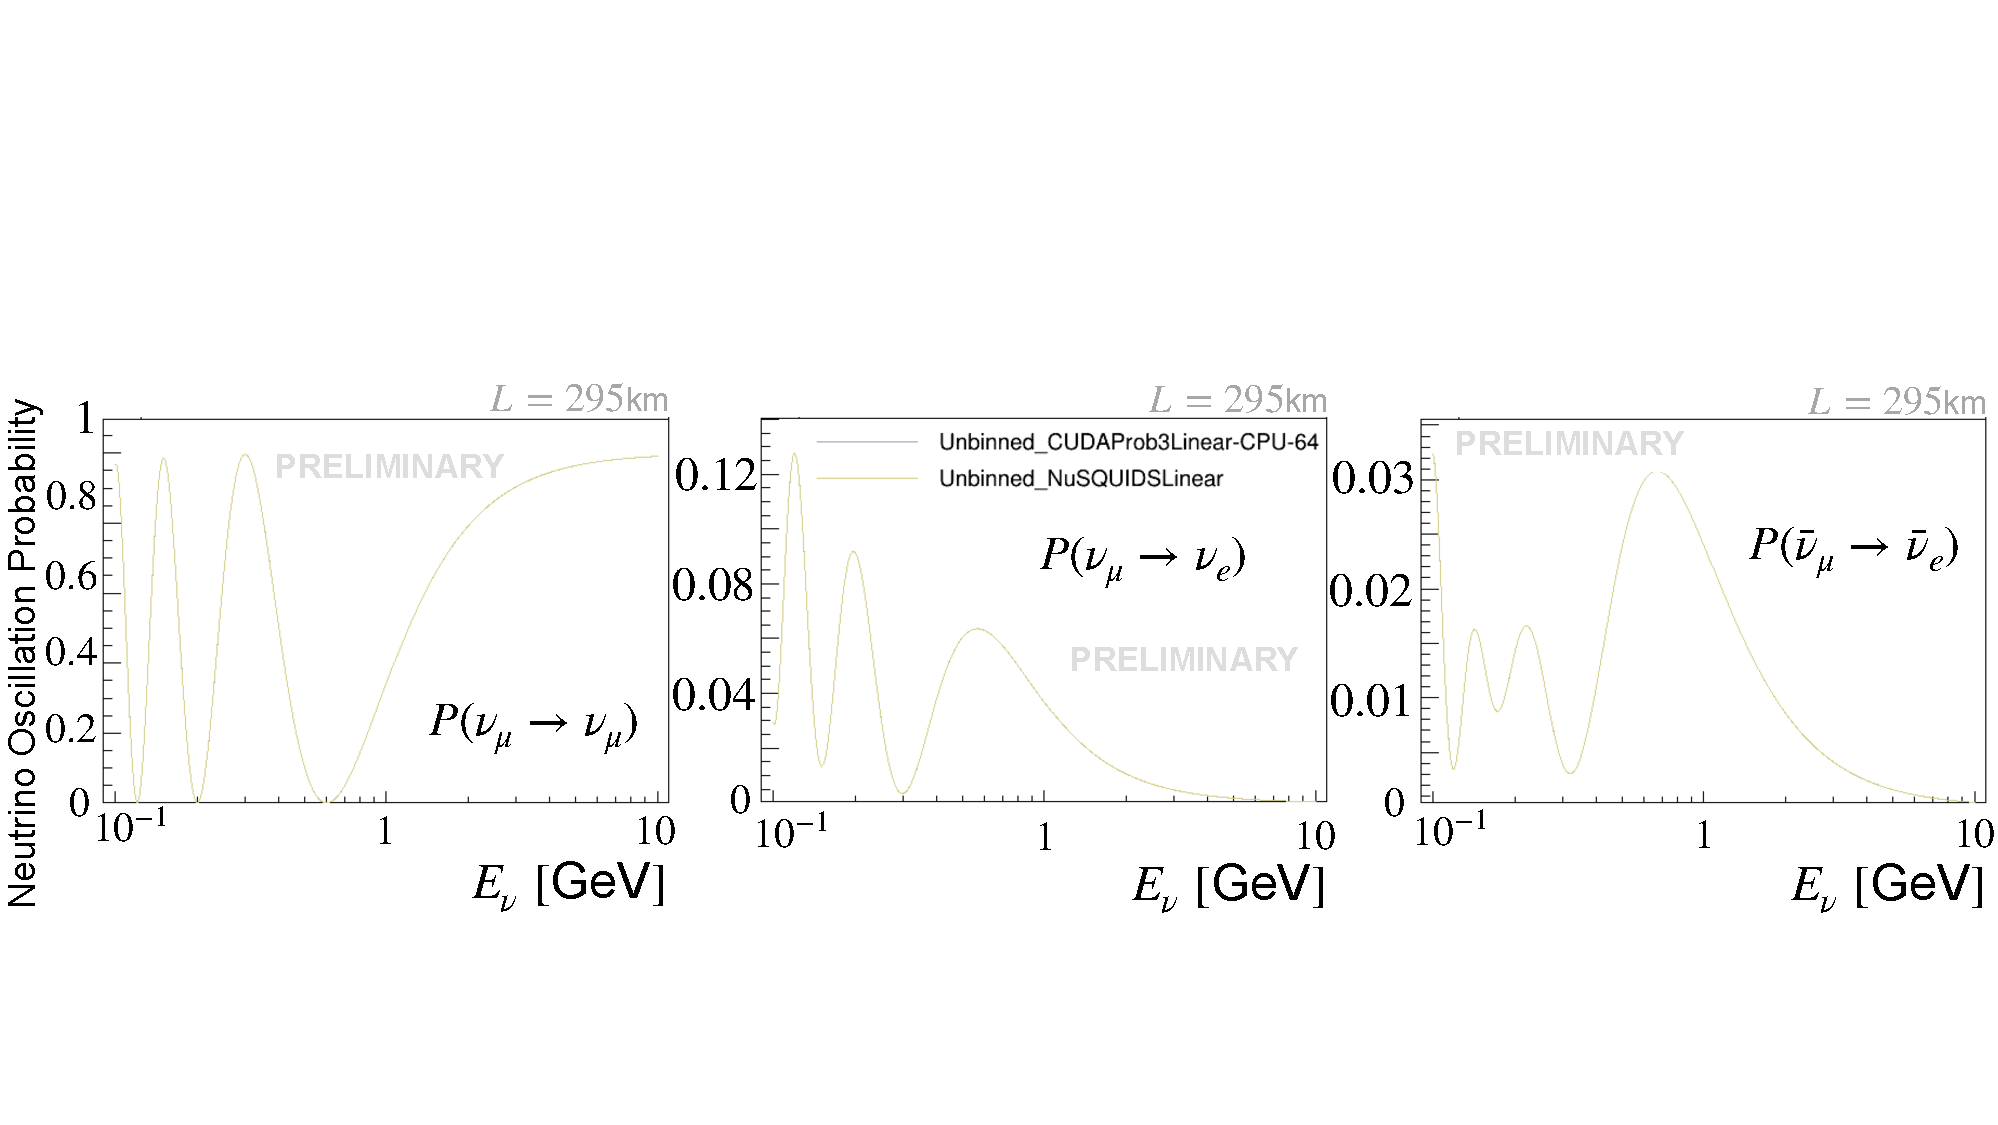
\includegraphics[width=1.\textwidth]
    {figures/osc_probs_validation2.pdf}
    %{figures/osc_probs_validation.pdf}
	\caption{Validation of the implementation of \acrshort{nusquids} into NuOscillator which is accesible by \acrshort{mach3}. Shown are (left) the muon-to-muon disappearance channel $\nu_\mu \rightarrow \nu_\mu$, (center) the muon-to-electron appearance channel $\nu_\mu \rightarrow \nu_e$ and (right) the muon-to-electron anti-neutrino appearance channel $\bar{\nu}_\mu \rightarrow \bar{\nu}_e$. The alternative model neutrino oscillation probabilities  with $\Gamma=0$ GeV (as shown in green) is overlaid with the \acrshort{sm} $3\times 3$-\acrshort{pmns} prediction (shown in blue). The other oscillation channels are not shown, but were validated in the same way.}
	\label{fig:osc_prob_validation}
    \end{figure}
%

\acrfull{nusquids} is designed to semi-analytically solve the evolution of density matrices and functions describing a collection of particles. It uses standard ordinary differential equations solvers via the standard GNU Scientific Library. \acrshort{nusquids} has been used by the IceCube collaboration to probe quantum gravitational signatures leading to decoherence for atmospheric neutrinos \cite{ICECUBE:2023gdv}. The implemented models in NuSQUIDS (with 3 neutrino flavours) are:
\begin{itemize}
    \item \acrshort{sm} neutrino oscillations (Standard 3x3 PMNS)
    \item \acrfull{qd}
    \item \acrfull{liv}
    \item \acrfull{nsi}
    \item \acrshort{sm} extension with sterile neutrino(s) (with $3+n_s$ neutrino flavours)
\end{itemize}
%
In total, there are $12$ parameters for fitting the neutrino oscillation probability in the quantum decoherence models. The Standard ($3\times3$-PMNS) neutrino oscillation parameters used to parametrise the matrix in \Cref{nu_osc_prob} are the neutrino mixing angles (usually expressed as the sines squared of the angle) $\sin^2(\theta_{12}), \sin^2(\theta_{23}), \sin^2(\theta_{13})$, the squared-mass differences $\Delta m^2_{12}$, $\Delta m^2_{23}$ where $\Delta m_{ij}^2 = m_i^2 - m_j^2$ [GeV$^2$] and the \acrfull{cp}-violating phase $\delta_{CP}$. The neutrino propagation and interaction parameters are the path lengths $l_\text{path}$ [km], i.e. for accelerator-neutrinos the baseline of the experiment, the Earth density $\rho_\oplus$ [g/cm$^3$] and the number of electrons per nucleon in a neutral atom (in the jargon referred to as electron density) $\rho_\text{e} = \frac{Z}{A}$ where $Z$ is the atomic (proton) number and $A$ is the mass (protons and neutrons) number. As mentioned in \Cref{subsec:oqsf}, the neutrino BSM quantum decoherence oscillation parameters are the decoherence strength $\Gamma(E_0)$ [GeV] and the energy scale $n$. The reference energy $E_0$ [GeV] is chosen to fix the energy reference scale of the energy considered in the analysis. The oscillation parameters are shown in \Cref{tab:qd_osc_params}.%\Cref{fig:qd_osc_params}.
\iffalse%
    \begin{figure}[H]
	\centering
    \includegraphics[width=1.\textwidth]{figures/qd_osc_params.png}
	\caption{Parameter choices and inputs for \acrshort{mach3}. The neutrino oscillation parameter choices are taken from the current oscillation analyses in \acrshort{dune} and \acrshort{t2k}, respectively.}
	\label{fig:qd_osc_params}
    \end{figure}
\fi%
%
\begin{table}[H]
    \centering
    \caption[]{Neutrino standard (3×3-\acrshort{pmns}) oscillation parameters $\sin^2(\theta_{12})$, $\sin^2(\theta_{23})$, $\sin^2(\theta_{13})$ (dimensionless), $\Delta m^2_{12}$ [GeV$^2$], $\Delta m^2_{23}$ [GeV$^2$], $\delta_\text{CP}$ [rad]; Neutrino propagation/interaction parameters $l_\text{path}$ [km], $\rho_\oplus$ [g/cm$^3$], $\rho_\text{e}$ (dimensionless); and the BSM quantum decoherence parameters $\Gamma$ [GeV], $n$ (dimensionless), and $E_0$ [GeV].}
    \label{tab:qd_osc_params}
    \resizebox{\columnwidth}{!}{%
        \begin{tabular}{|l||c|c|c|c|c|c||c|c|c||c|c|c|}
        \hline
        \begin{tabular}{c}\textbf{Oscillation}\\[-1mm]\textbf{Parameters}\end{tabular} & 
            \begin{tabular}{c}$\sin^2(\theta_{12})$\\[-1mm] \scriptsize{[ - ]}\end{tabular} &
            \begin{tabular}{c}$\sin^2(\theta_{23})$\\[-1mm] \scriptsize{[ - ]}\end{tabular} &
            \begin{tabular}{c}$\sin^2(\theta_{13})$\\[-1mm] \scriptsize{[ - ]}\end{tabular} & 
            \begin{tabular}{c}$\Delta m^2_{12}$\\[-1mm] \scriptsize{[GeV$^2$]}\end{tabular} &
            \begin{tabular}{c}$\Delta m^2_{23}$\\[-1mm] \scriptsize{[GeV$^2$]}\end{tabular} &
            \begin{tabular}{c}$\delta_\text{CP}$\\[-1mm] \scriptsize{[rad]}\end{tabular} &
            \begin{tabular}{c}$l_\text{path}$\\[-1mm] \scriptsize{[km]}\end{tabular} &
            \begin{tabular}{c}$\rho_\oplus$\\[-1mm] \scriptsize{[g/cm$^3$]}\end{tabular} &
            \begin{tabular}{c}$\rho_\text{e}$\\[-1mm] \scriptsize{[ - ]}\end{tabular} &
            \begin{tabular}{c}$\Gamma$\\[-1mm] \scriptsize{[GeV]}\end{tabular} &
            \begin{tabular}{c}$n$\\[-1mm] \scriptsize{[ - ]}\end{tabular} &
            \begin{tabular}{c}$E_0$\\[-1mm] \scriptsize{[GeV]}\end{tabular}
            \\ \hline \hline
            \textbf{\acrshort{dune}} & $0.307$ & $0.528$ & $0.0218$ & $7.53\times10^{-5}$ & $2.509\times10^{-3}$ & $-1.6$ & $1284.9$ & $2.848$ & $0.5$ & $9.48\times10^{-18}$ & $2$ & $1.0$ \\ \hline
            \textbf{\acrshort{t2k}} & $0.307$ & $0.561$ & $0.0220$ & $7.53\times10^{-5}$ & $2.494\times10^{-3}$ & $-1.6$ & $295.0$ & $2.6$ & $0.5$ & $9.48\times10^{-18}$ & $2$ & $1.0$ \\ \hline
        \end{tabular}
    }
\end{table}


\subsection{Quantum Decoherence in \texorpdfstring{\acrshort{dune}}{TEXT} and \texorpdfstring{\acrshort{t2k}}{TEXT}} \label{sec:qd_param_choices}
%
The decoherence matrix $D$ in \Cref{eq:decoherence_operator} produces damping terms of the form $e^{-\Gamma L}$. The coherence length $L_\text{coh}$ is referred to as the distance at which damping terms have reached $e^{-1}$, which implies:
\vspace{-3mm}%
\begin{align} \label{decoherence_length}
   L_\text{coh} = \frac{1}{\Gamma(E^\text{ref}_\nu)} \ .
\end{align}
%
Eq. (\ref{decoherence_length}) can be interpreted as the neutrino interaction mean free path and allows an estimate of the decoherence strength $\Gamma(E_\nu)$ at a reference energy $E^\text{ref}_\nu$. For example, using \Cref{decoherence_length} and setting the \acrshort{dune} baseline of $1284.8 \ $km to $L_\text{coh}$ yields a decoherence strength of
\vspace{-3mm}%
\begin{align} \label{decoherence_strength_dune}
   \Gamma\left(\bigl \langle E^\text{\acrshort{dune}}_\nu \bigr \rangle \right) = \frac{\hbar c}{l^\text{\acrshort{dune}}_\text{baseline}} = \frac{0.197 \ \text{GeV fm}}{1.2849 \cdot 10^{21} \ \text{fm}} \approx 1.534 \cdot 10^{-22} \ \text{GeV}  \ \text{,}
\end{align}
%
and the T$2$K baseline of $295 \ $km yields a decoherence strength of
\vspace{-3mm}%
\begin{align} \label{decoherence_strength_t2k}
   \Gamma\left(\bigl \langle E^\text{\acrshort{t2k}}_\nu \bigr \rangle \right) = \frac{\hbar c}{l^\text{\acrshort{t2k}}_\text{baseline}} = \frac{0.197 \ \text{GeV fm}}{2.95 \cdot 10^{20} \ \text{fm}} \approx 6.678 \cdot 10^{-22} \ \text{GeV}  \ .
\end{align}
%
This estimate for the decoherence strength with respect to a reference energy then allows to find an estimate of the constant decoherence strength parameter $\Gamma(E_0)$, whose magnitude is fixed by the arbitrarily chosen pivot point energy $E_0$. We can rearrange \Cref{gamma-parameter} with $n=1$ to find an estimate for $\Gamma(E_0)$:
\vspace{-3mm}%
%
\begin{align} \label{decoherence_strength_frac}
   \frac{\Gamma(E_\nu)}{E_\nu} = \frac{\Gamma(E_0)}{E_0} .
\end{align}
%
For example, taking the mean neutrino flux energy $\bigl \langle E^\text{\acrshort{dune}}_\nu \bigr \rangle = 2\ $GeV for \acrshort{dune}, and $\bigl \langle E^\text{\acrshort{t2k}}_\nu \bigr \rangle = 0.6 \ $GeV for \acrshort{t2k} and other reference energies for comparison, we find the combinations of parameters as listed in \Cref{tab:params} that result in the same decoherence effect.
%
%\ohead{\ref{sec:qd_param_choices} Quantum Decoherence in DUNE / T2K}
%
%
\begin{table}[htb]
	\caption[]{Quantum decoherence parameter choices for the decoherence strength $\Gamma(E_0)$, energy scale $n$ and reference energy $E_0$ that lead to the same decoherence effect. The neutrino oscillation parameters are chosen as stated in \Cref{tab:qd_osc_params}.} \label{tab:params}
    \resizebox{\textwidth}{!}{%
	\begin{tabular}{|l||c|}
		\hline
		\diagbox{$E^\text{ref}_\nu$}{\text{Parameter}} & $\bigl\{ \Gamma(E_0) \ [\text{GeV}],n, E_0 \ [\text{GeV}] \bigr\}$ \\ \hline \hline
            $\bigl \langle E^\text{\acrshort{dune}}_\nu  \bigr \rangle = 2\ \text{GeV}$    & $\{7.67\cdot 10^{-23}, \ 1, \ 1.0\}$, $\{1.53\cdot 10^{-22}, \ 1, \ 2.0\}$, $\{7.67\cdot 10^{-22}, \ 1, \ 10.0\}$ \\ \hline
            $\bigl \langle E^\text{\acrshort{dune}}_\nu  \bigr \rangle = 2\ \text{GeV}$    & $\{3.84\cdot 10^{-23}, \ 2, \ 1.0\}$, $\{1.53\cdot 10^{-22}, \ 2, \ 2.0\}$, $\{3.84\cdot 10^{-21}, \ 2, \ 10.0\}$ \\ \hline  
            $\bigl \langle E^\text{\acrshort{t2k}}_\nu  \bigr \rangle = 0.6\ \text{GeV}$    & $\{1.11\cdot 10^{-21}, \ 1, \ 1.0\}$, $\{2.23\cdot 10^{-21}, \ 1, \ 2.0\}$, $\{1.11\cdot 10^{-20}, \ 1, \ 10.0\}$ \\ \hline
            $\bigl \langle E^\text{\acrshort{t2k}}_\nu  \bigr \rangle = 0.6\ \text{GeV}$    & $\{1.85\cdot 10^{-21}, \ 2, \ 1.0\}$, $\{7.42\cdot 10^{-21}, \ 2, \ 2.0\}$, $\{1.85\cdot 10^{-20}, \ 2, \ 10.0\}$ \\ \hline
            $5\ \text{GeV}$    & $\{1.34\cdot 10^{-22}, \ 1, \ 1.0\}$, $\{2.67\cdot 10^{-22}, \ 1, \ 2.0\}$, $\{1.23\cdot 10^{-21}, \ 1, \ 10.0\}$ \\ \hline
            $20\ \text{GeV}$    & $\{7.67\cdot 10^{-24}, \ 1, \ 1.0\}$, $\{1.53\cdot 10^{-23}, \ 1, \ 2.0\}$, $\{7.67\cdot 10^{-23}, \ 1, \ 10.0\}$ \\ \hline
	\end{tabular}
    }
\end{table} 
%
\iffalse
%
\begin{wrapfigure}{r}{0.45\textwidth}
	\vspace{-12mm}
	\begin{center}
		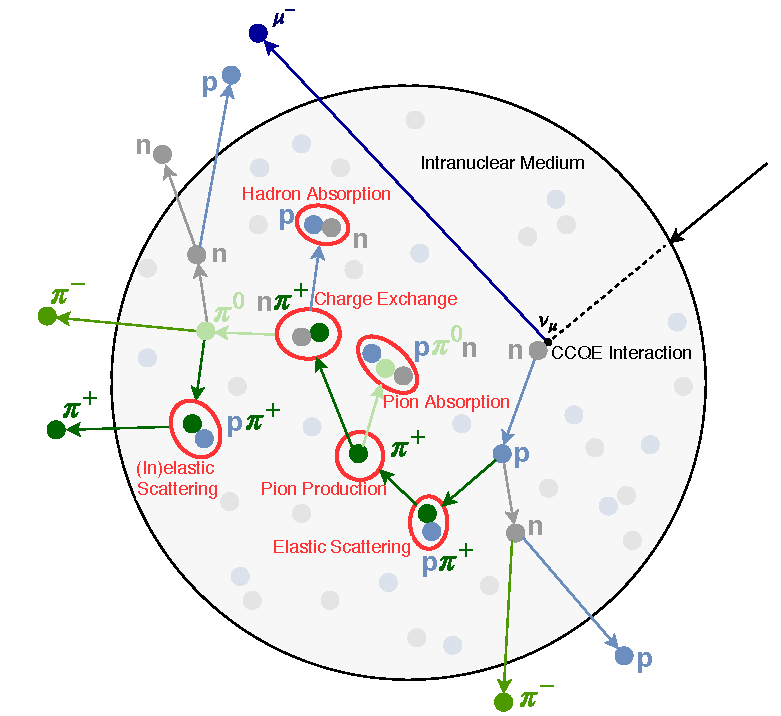
\includegraphics[width=0.45\textwidth]{figures/FSIs.pdf}
	\end{center}
	\vspace{-7mm}
	\caption[Illustration of Final-State Interactions]{Final-State Interactions. %in an intranuclear cascade model approach. %The incoming muon neutrino $\nu_\mu$ represented by the black arrow followed by the dashed black line interacts via a charged-current quasi-elastic interaction with a neutron in an argon nucleus.
	%The outgoing muon (indigo line) and proton (light blue line) traverse the nuclear medium. The proton can undergo various types of hadronic FSIs such as (in)elastic scattering, pion production, hadron absorption and charge exchange. Pions in this figure are shown in dark green ($\pi^+$), regular green ($\pi^-$), and light green ($\pi^0$).
    }
	\vspace{4mm}
	\label{FSIs}
\end{wrapfigure}
%
\fi
%
The parameter choices in \Cref{sec:results} are such that one can observe the effect of decoherence on the predicted event rates in \acrshort{dune} and \acrshort{t2k}. Note, that a more careful analysis is needed in order to make predictions on what can actually be observed in \acrshort{dune} or \acrshort{t2k}. The parameter combinations given in \Cref{tab:qd_osc_params} are indicators for the order of magnitude of $\Gamma(E_0)$. Ultimately, observing the damping as described in \Cref{decoherence_length} requires choosing a $\mathcal{D}[\rho]$ in \Cref{eq:lindblad-master-eq} such that the damping terms act uniformly on all components contributing to the neutrino oscillation probability.


\subsection{Decoherence Strength Variations}
%\ohead{\headmark}
The event rate predictions in the \acrlong{fd}s of \acrshort{dune} and \acrshort{t2k} for the available \acrshort{cc}$\overset{\brobor}{\nu}_\mu$ samples are shown in figs. \ref{fig:qd_dune_numu_gamma_varied} and \ref{fig:qd_t2k_gamma_varied}, respectively, while the predictions for the \acrshort{cc}$\overset{\brobor}{\nu}_e$ samples in \acrshort{dune} for varying $\Gamma(E_0)$ are shown in \Cref{fig:qd_dune_nue_gamma_varied}. The number of \acrshort{cc}$\overset{\brobor}{\nu}_\mu$ events for varying $n$ are shown in \Cref{fig:qd_dune_numu_n_varied}.
%
    \begin{figure}[hp]
	\centering
	%\includegraphics[width=1.\textwidth]{figures/QD_DUNEnumu_Gamma_varied.pdf}
    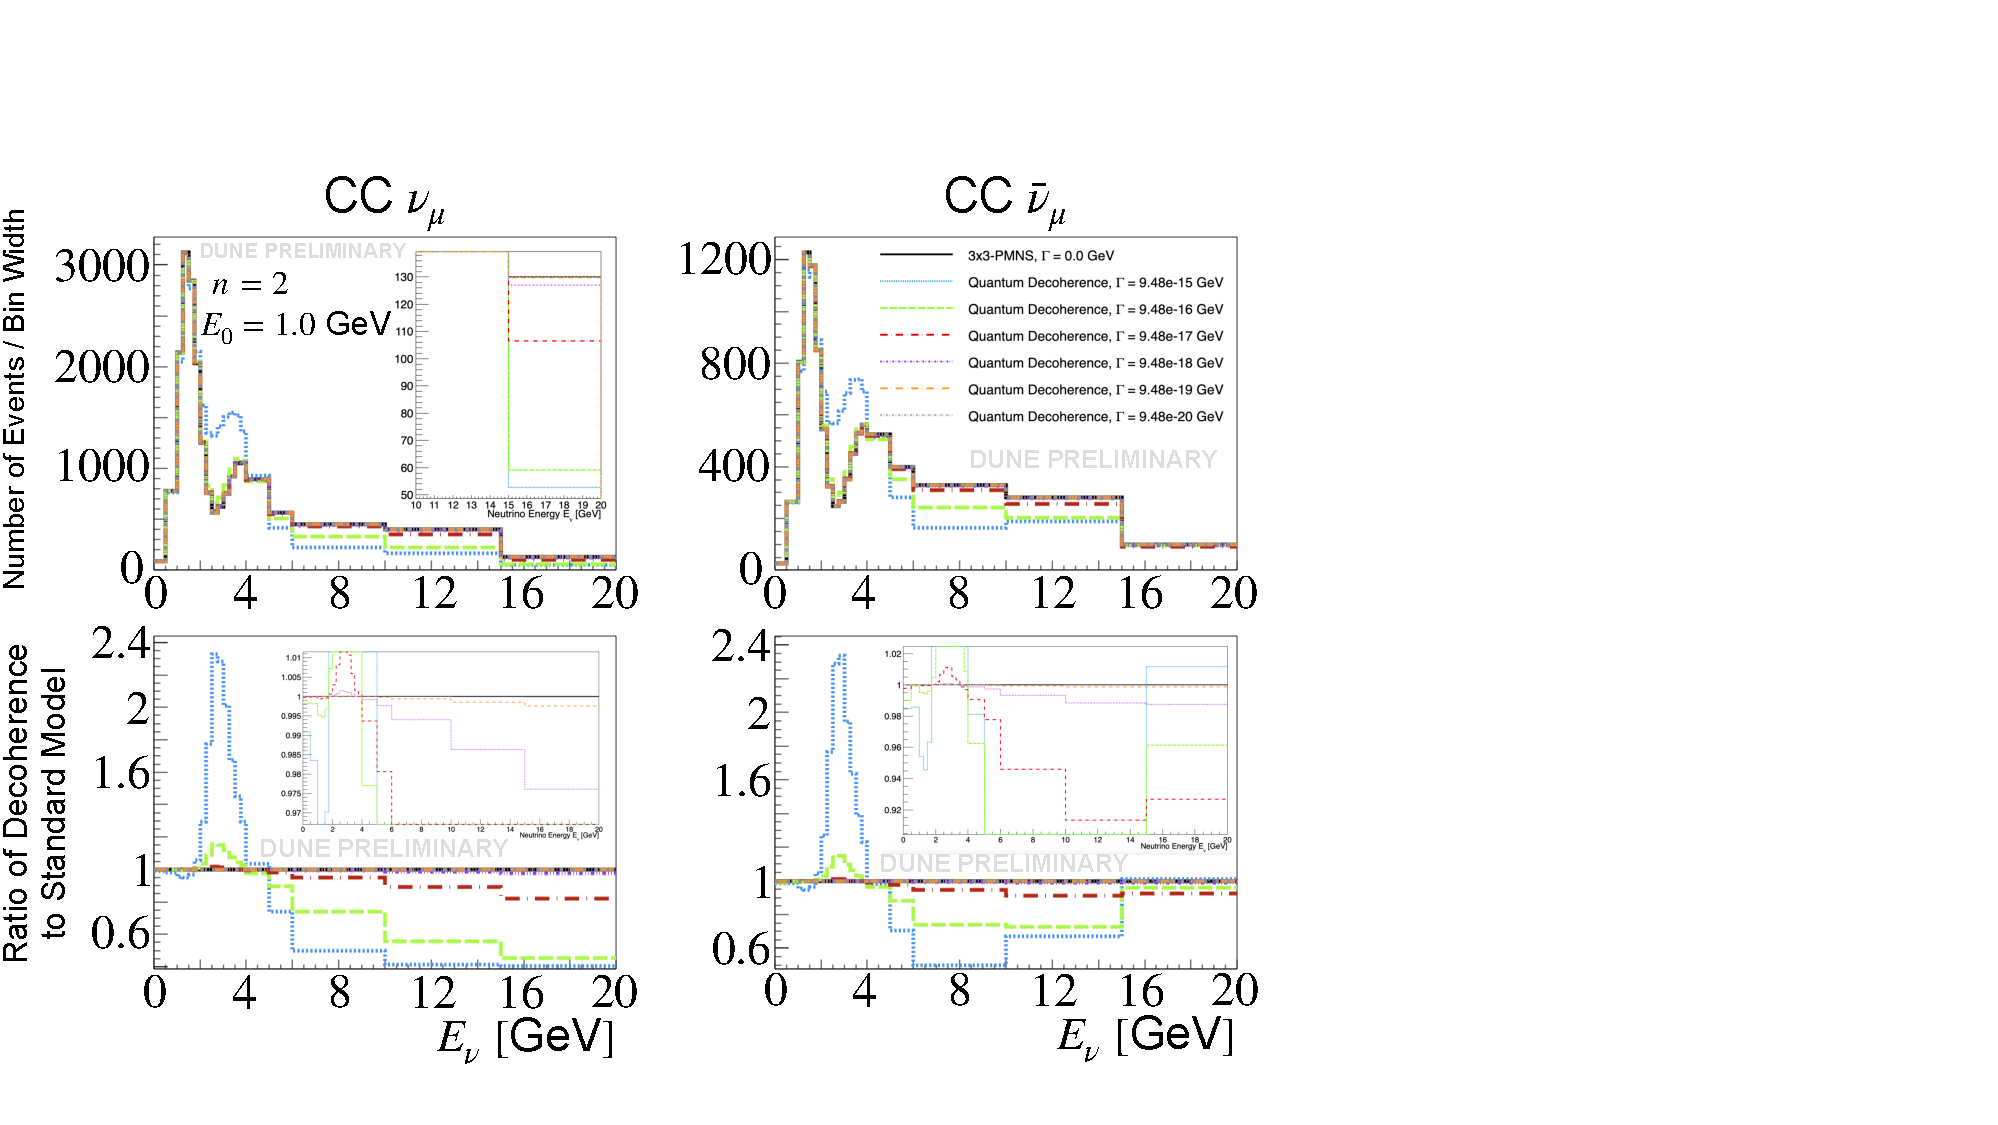
\includegraphics[width=1.\textwidth]{figures/QD_DUNEnumu_Gamma_varied2.pdf}
	\caption{Upper row: Muon neutrino and anti-neutrino event rates in \acrshort{dune}. Lower row: Ratios of the decoherence to standard model event rates of the plots above, respectively. In the plots shown, the decoherence strength $\Gamma(E_0)$ is varied while the energy scale is fixed at $n=2$.}
	\label{fig:qd_dune_numu_gamma_varied}
    \end{figure}
%
% DUNE plots
%\vspace{-5mm}
%
    \begin{figure}[tp]
	\centering
	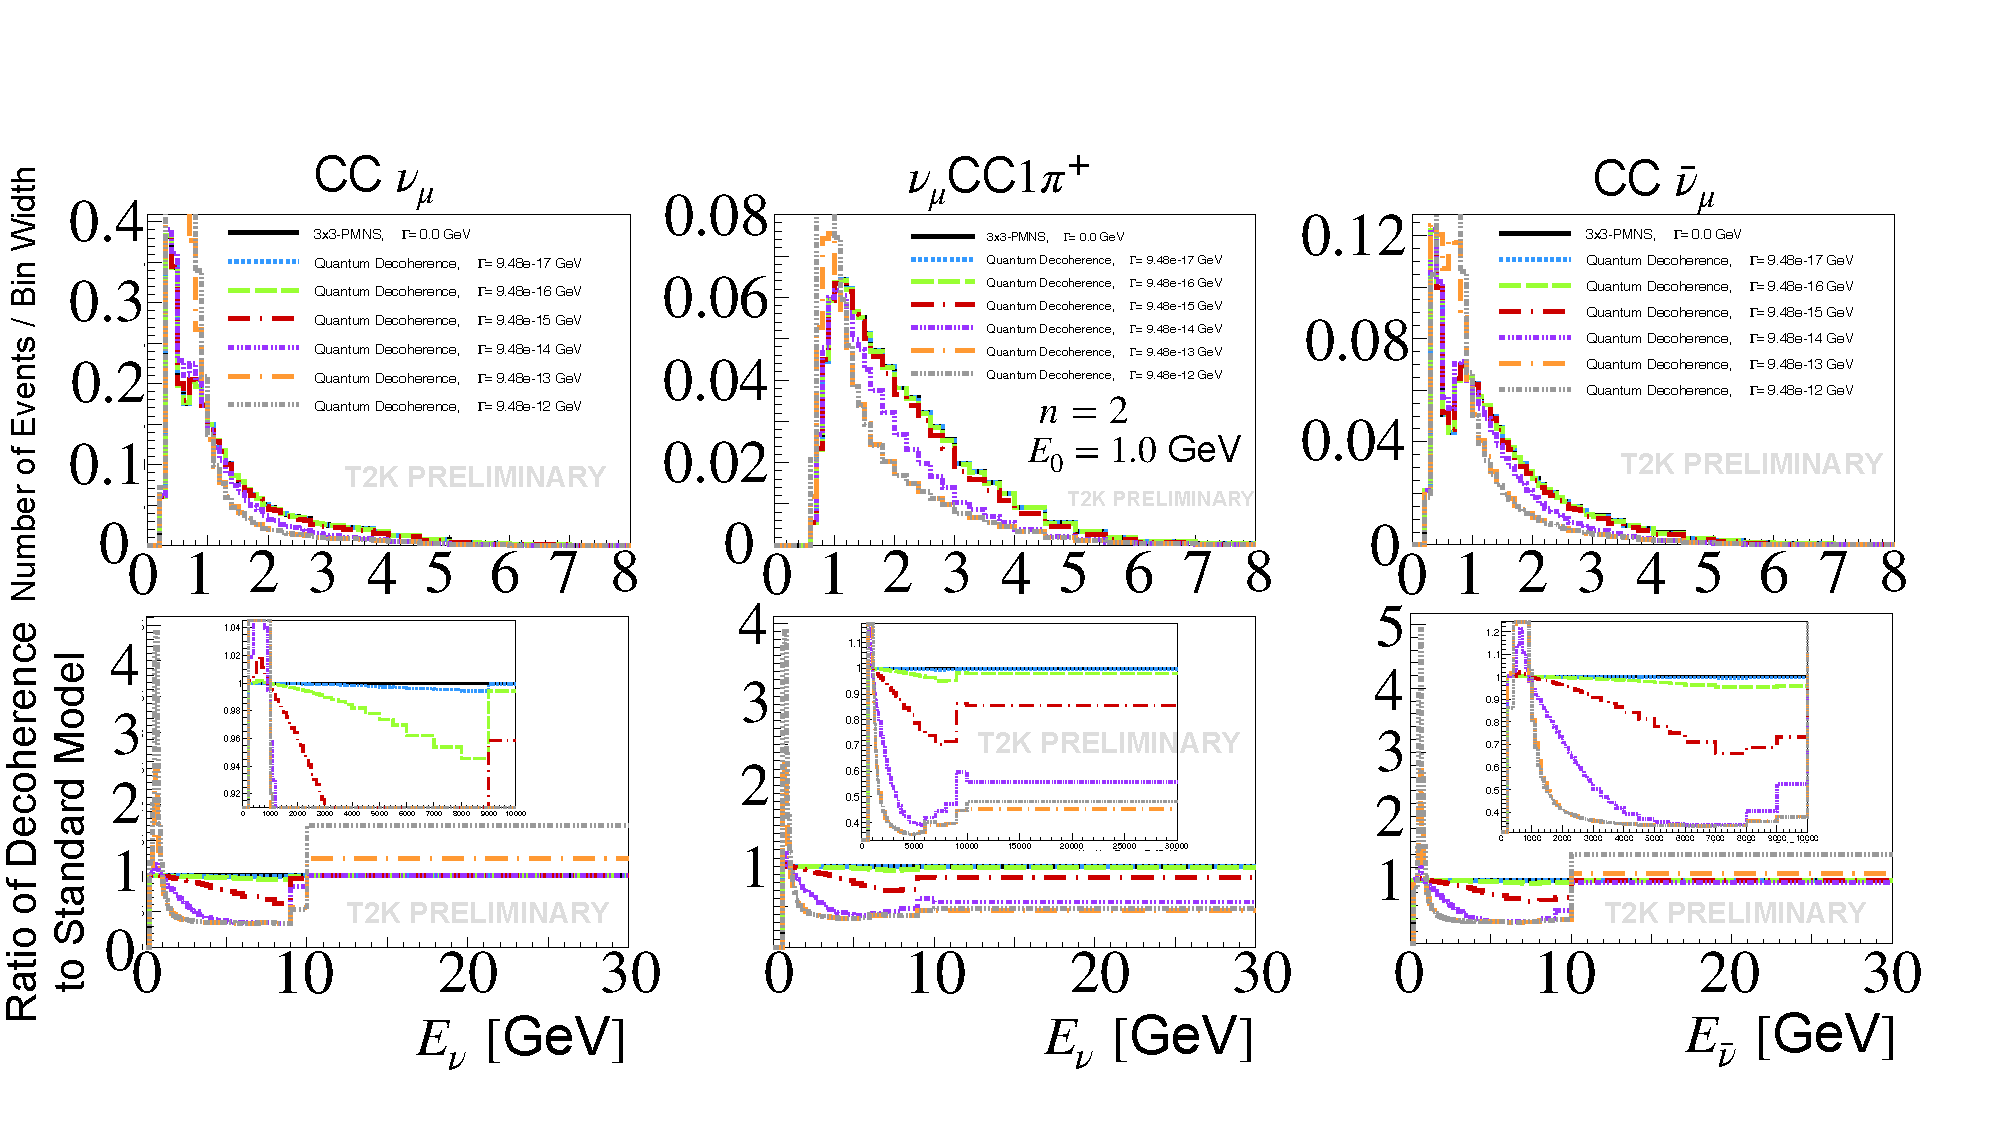
\includegraphics[width=1.\textwidth]
    {figures/QD_T2K_Gamma_varied2.pdf}
    %{figures/QD_T2K_Gamma_varied.pdf}
	\caption{Upper row: Muon neutrino and anti-neutrino event rates in \acrshort{t2k}. The middle column shows a sample in which there is an additional pion produced in the neutrino interaction. Lower row: Ratios of the decoherence to standard model event rates of the plots above, respectively. In the plots shown, the decoherence strength $\Gamma(E_0)$ is varied while the energy scale is fixed at $n=2$.
    }
	\label{fig:qd_t2k_gamma_varied}
    \end{figure}
%
The plots in figs. \ref{fig:qd_dune_numu_gamma_varied} and \ref{fig:qd_dune_nue_gamma_varied} show how the event range changes with varying decoherence strength parameter $\Gamma(E_0)$ for a particular choice of the energy scale $n = 2$ in \acrshort{dune}. The ratio of the event rates of the decoherence to the standard model predictions are shown underneath the event rate plots. The \acrshort{sm} predicted event rate is shown alongside the alternative model predictions in black, which corresponds to the case where the decoherence effect is turned off ($\Gamma = 0$ GeV). Since this choice of $n=2$ means a quadratic dependence of the decoherence effect on the neutrino energy $E_\nu$, one can see in all plots shown in figs. \ref{fig:qd_dune_numu_gamma_varied} and \ref{fig:qd_dune_nue_gamma_varied} that there are larger deviations with increasing reconstructed neutrino energy from the \acrshort{sm} $3 \times 3$-\acrshort{pmns} neutrino oscillation probability. In particular, it is interesting to note that decoherence enhances the relative number of \acrshort{cc}$\overset{\brobor}{\nu}_\mu$ events (\Cref{fig:qd_dune_numu_gamma_varied}) and it decreases the relative number of \acrshort{cc}$\overset{\brobor}{\nu}_e$ events (\Cref{fig:qd_dune_nue_gamma_varied}).
%
    \begin{figure}[hbt]
	\centering
	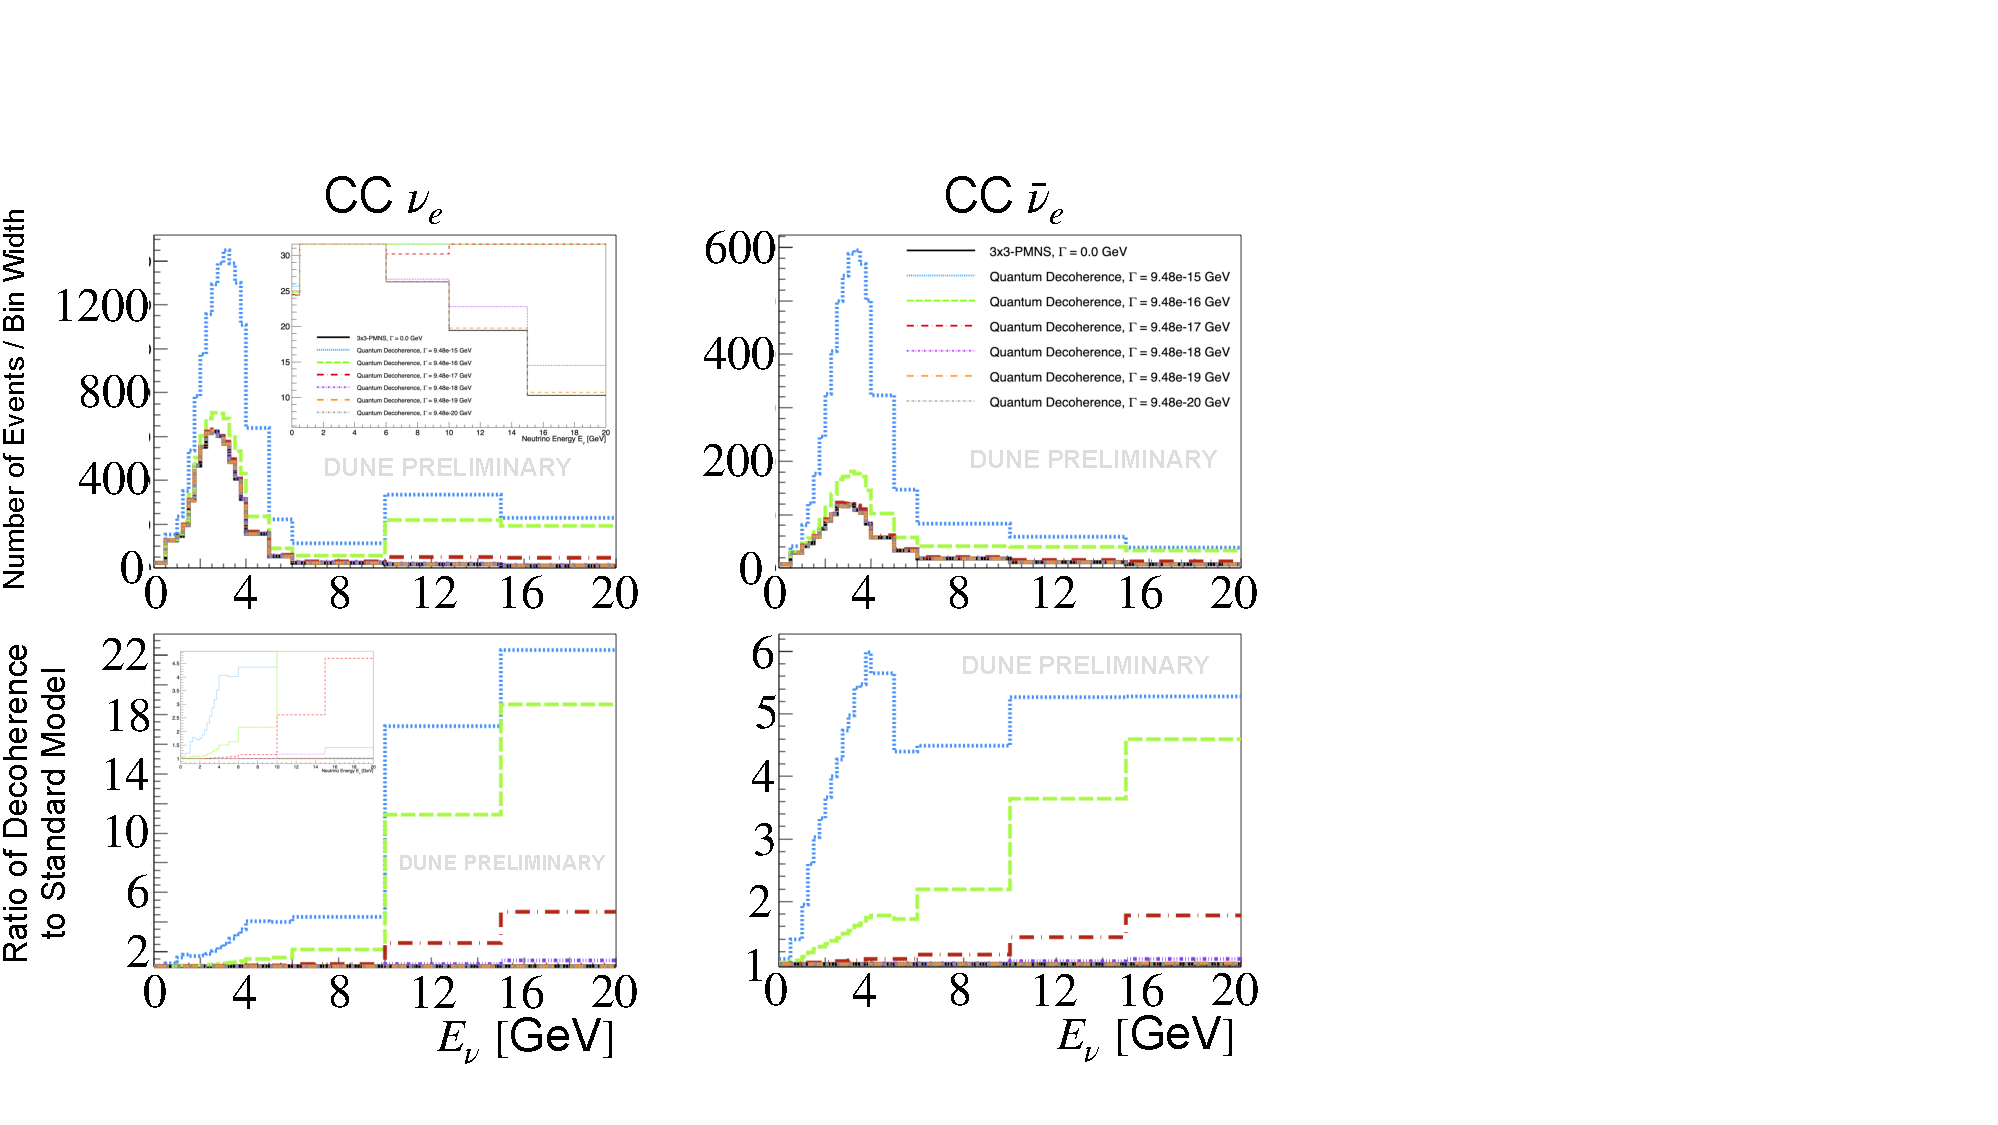
\includegraphics[width=1.\textwidth]{figures/QD_DUNEnue_Gamma_varied.pdf}
	\caption{Upper row: Electron neutrino and anti-neutrino event rates in \acrshort{dune}. Lower row: Ratios of the decoherence to standard model event rates of the plots above, respectively. In the plots shown, the decoherence strength $\Gamma(E_0)$ is varied while the energy scale is fixed at $n=2$.}
	\label{fig:qd_dune_nue_gamma_varied}
    \end{figure}
%
This can be especially seen in the inlets of the ratio plots. For example, the decoherence strength set to a standard value in the literature of $\Gamma(E_0) = 9.48\times10^{-18}$ GeV leads to a $2.4\%$ reduction in the highest reconstructed neutrino energy bin shown (close to $20$ GeV) for muon-neutrinos and a $1.2\%$ variation in for muon anti-neutrinos. In the highest energy bin, decoherence increases the number of relative events by $40\%$ for electron-neutrinos and by $9.8\%$ for electron anti-neutrinos.

% T2K plots
The same qualitative observations apply to the \acrshort{t2k} event rates, yet the same choices of $\Gamma(E_0)$ do not lead to the same strength of the effect in the case of $n=2$. This is due to the \acrshort{t2k} flux exhibiting less-energetic neutrinos compared to \acrshort{dune}. The analogous plots with respect to \Cref{fig:qd_dune_numu_gamma_varied} for \acrshort{dune} are shown in \Cref{fig:qd_t2k_gamma_varied} for \acrshort{t2k}. The dip between the two peaks in the muon neutrino sample around $600$ MeV is due to muon-neutrinos oscillating away from being muon-neutrinos as can be read-off the muon-neutrino disappearance probability $P_{\nu_\mu \rightarrow \nu_\mu}$ on left in \Cref{fig:osc_prob_validation}. It can be seen that decoherence effects increase the number of events in the low-energy region (due to the majority of events originating from electron-neutrino interactions). The following second peak around $700$ MeV is dominated by muon-neutrino events where decoherence effects decrease the number of events for these higher energies (due to the majority of events originating from muon-neutrino interactions).
%
Whereas the decoherence effect assuming a quadratic energy dependence ($n=2$) is expected to cause larger variations at higher energies, the event rate histograms converge against the \acrshort{sm} prediction and eventually to zero in the higher energy region. This is due to the \acrshort{t2k} neutrino flux being less and less populated with increasing energy.

More details are shown in \Cref{fig:qd_t2k_gamma_varied_highlights1}. For the decoherence strength of an order of magnitude of $\Gamma(E_0) \sim \mathcal{O}\left(10^{-15} \text{ GeV}\right)$, there is a $5.5\%$ reduction in the reconstructed neutrino energy bin around $8$ GeV for muon-neutrinos and a $1.2\%$ increase for electron neutrinos. For $\Gamma(E_0) \sim \mathcal{O}\left(10^{-16} \text{ GeV}\right)$, there is a $0.6\%$ difference. For electron-neutrinos, decoherence increases the number of relative events by $0.1\%$ in the highest energy bin around $1.2$ GeV. ToDo: -> rething this part....
%
    \begin{figure}[hbt]
	\centering
	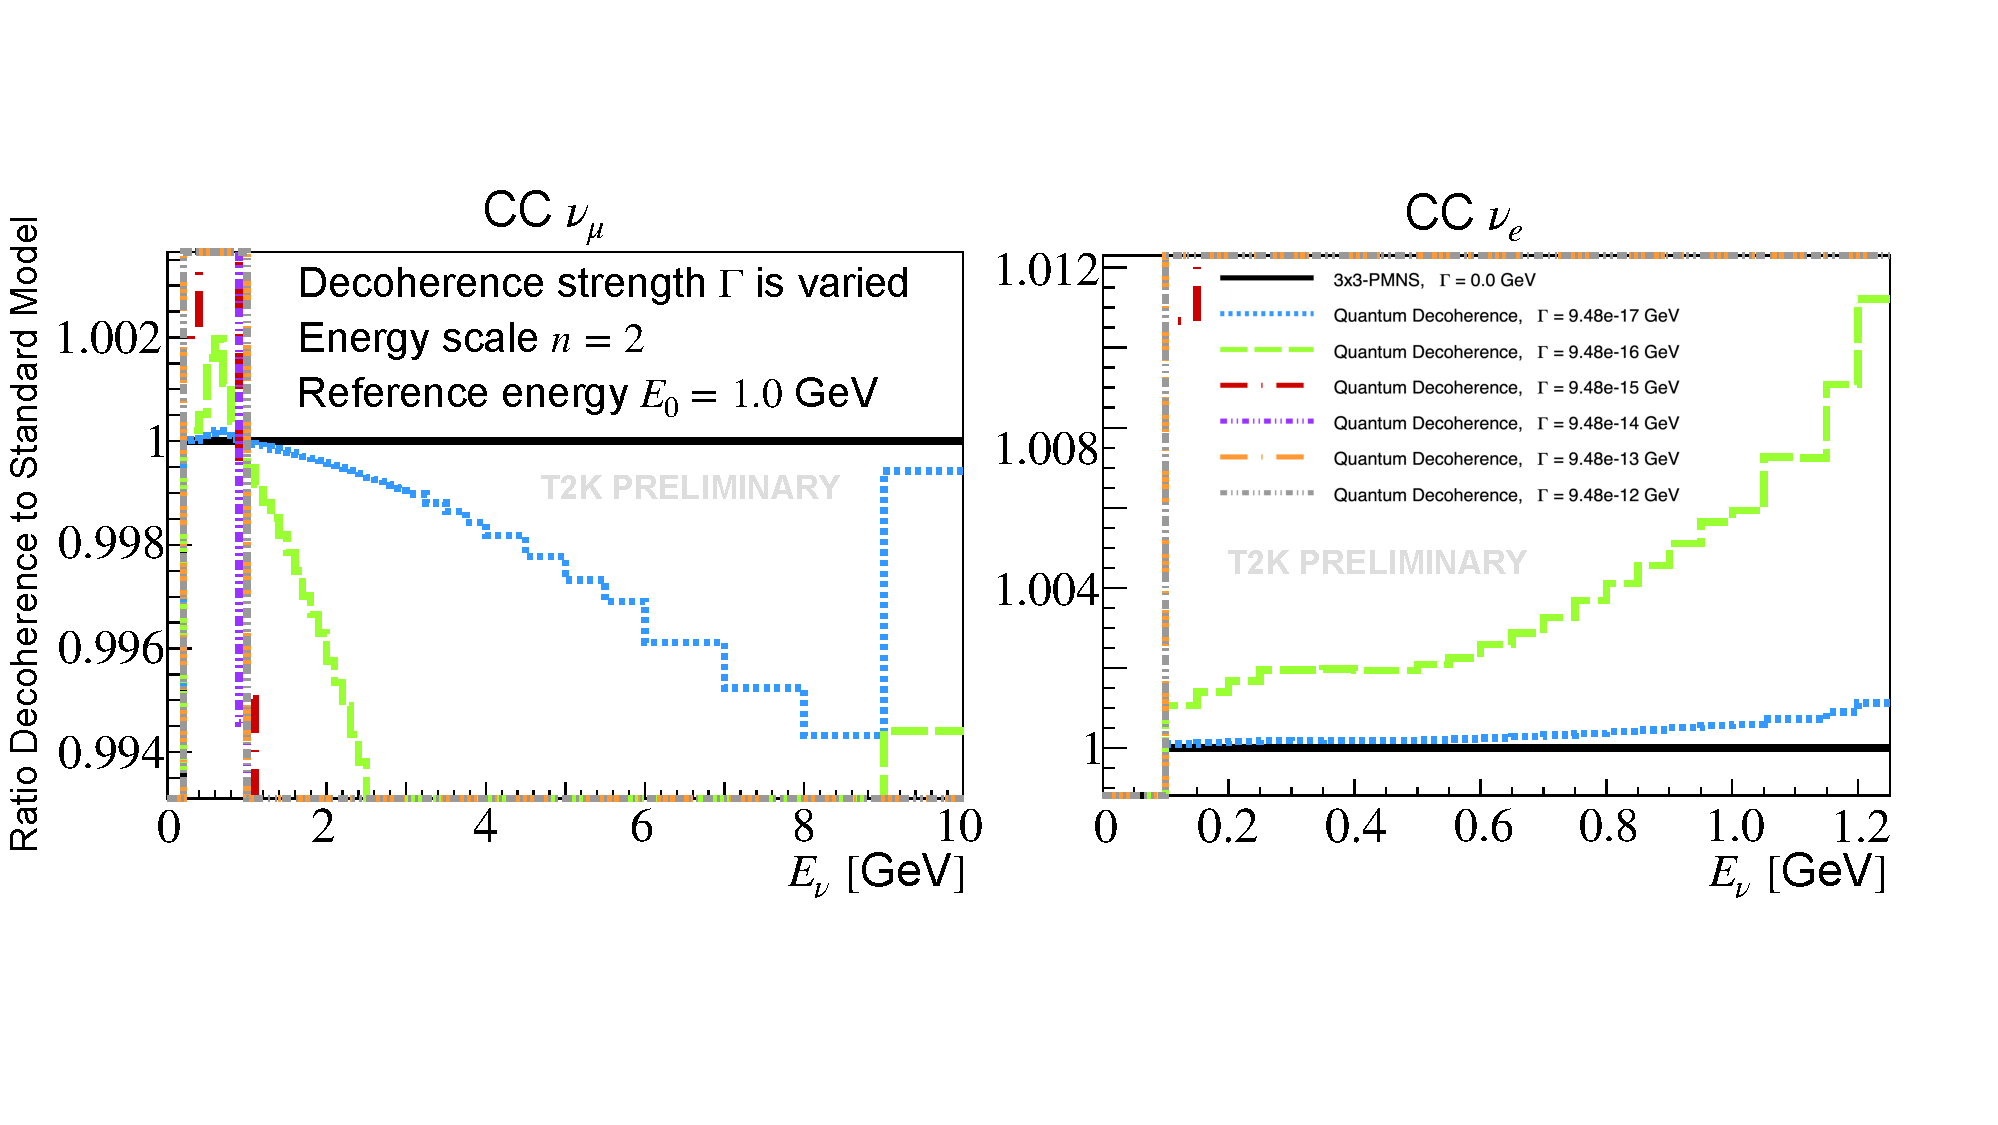
\includegraphics[width=1.\textwidth]
    {figures/QD_T2K_Gamma_varied_highlights_2.pdf}
    %{figures/QD_T2K_Gamma_varied_highlights.pdf}
	\caption{Left: Inlet of the \acrshort{cc} muon-neutrino event rate and right: of the \acrshort{cc} electron-neutrino event rate in \acrshort{t2k}. The decoherence strength $\Gamma(E_0)$ is varied while the energy scale exponent is fixed at $n=2$.}
	\label{fig:qd_t2k_gamma_varied_highlights1}
    \end{figure}
%

\subsection{Energy Scale Variations}
%\FloatBarrier
An inversely proportional quadratic energy dependence is investigated in \Cref{fig:qd_t2k_gamma_varied_highlights2}, in which the energy scale is set to $n=-2$. This case is supposedly more interesting in \acrshort{t2k} compared to the previous as the decoherence effect is expected to be more dominant at lower energies. In \Cref{fig:qd_t2k_gamma_varied_highlights2}, it can indeed be seen that largest variations in both the \acrshort{cc}$\nu_e$ and \acrshort{cc}$\bar{\nu}_e$ samples depicted show up at lower energies and then decrease with increasing energy. There is a $3.5\%$ variation for $\Gamma(E_0) \sim \mathcal{O}\left(10^{-15} \text{ GeV}\right)$ and a $0.5\%$ variation for $\Gamma(E_0) \sim \mathcal{O}\left(10^{-16} \text{ GeV}\right)$ for electron-neutrinos. For electron anti-neutrinos, the variation is $7\%$ for $\Gamma(E_0) \sim \mathcal{O}\left(10^{-15} \text{ GeV} \right)$ and $0.9\%$ for $\Gamma(E_0) \sim \mathcal{O}\left(10^{-16} \text{ GeV} \right)$.
%
    \begin{figure}[hbt]
	\centering
	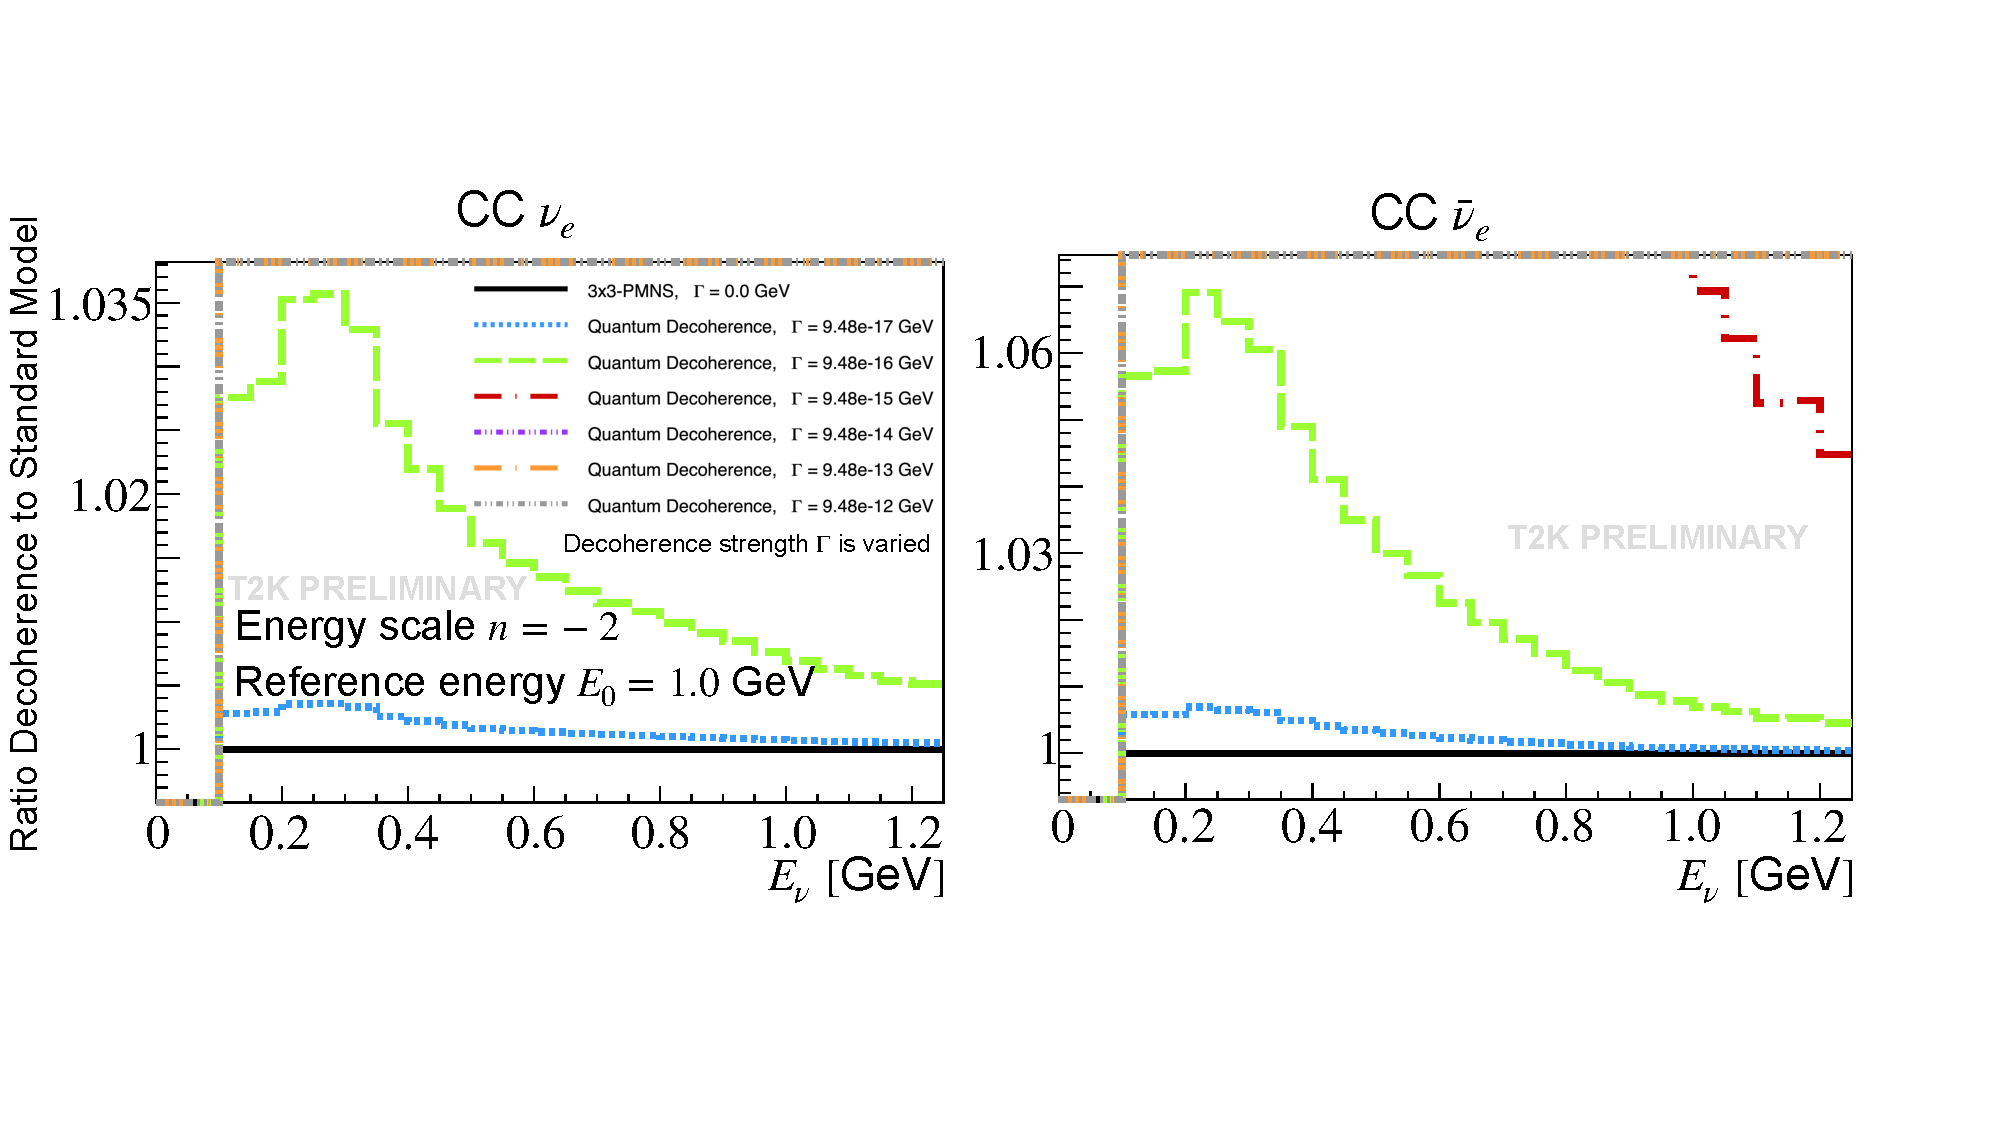
\includegraphics[width=1.\textwidth]
    {figures/QD_T2K_Gamma_varied_highlights2_2.pdf}
    %{figures/QD_T2K_Gamma_varied_highlights2.pdf}
	\caption{Left: Inlet of the \acrshort{cc} electron-neutrino event rate and right: of the \acrshort{cc} anti-electron-neutrino event rate in \acrshort{t2k}. The decoherence strength $\Gamma(E_0)$ is varied while the energy scale exponent is fixed at $n=2$.}
	\label{fig:qd_t2k_gamma_varied_highlights2}
    \end{figure}
%
The case where $\Gamma(E_0) = 9.48 \times 10^{-18}$ GeV and the energy scale $n$ is varied is shown in \Cref{fig:qd_dune_numu_n_varied} (\acrshort{dune}) and \Cref{fig:qd_t2k_n_varied} (\acrshort{t2k}). In the plots shown, the described qualitative enhancement of the decoherence effect for lower energies in case of negative $n$ and high energies for positive $n$ is clearly observable.
%
    \begin{figure}[hptb]
	\centering
	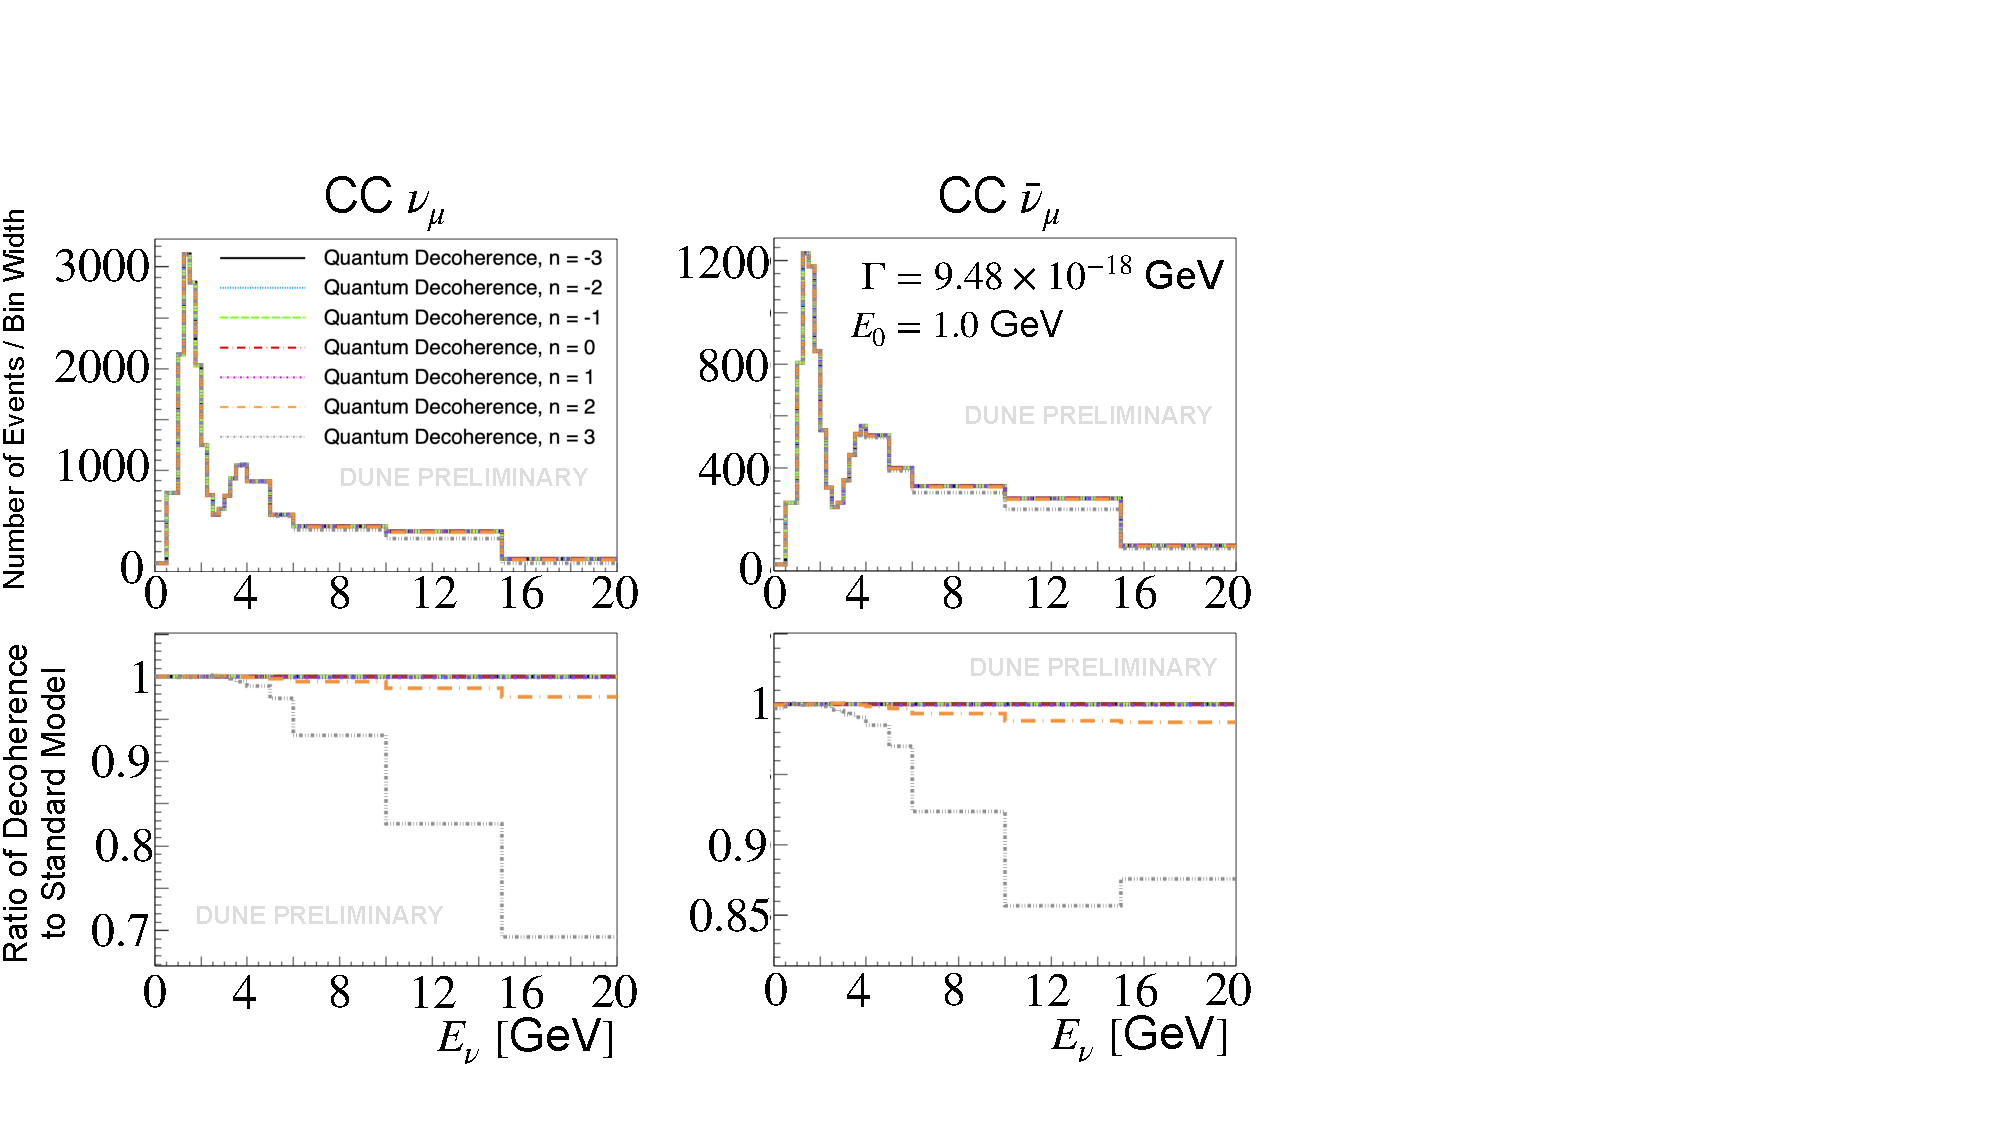
\includegraphics[width=1.\textwidth]{figures/QD_DUNEnumu_n_varied.pdf}
	\caption{Left: \acrshort{cc} muon-neutrino event rate and ratios. Right: \acrshort{cc} electron-neutrino event rate and ratios in \acrshort{dune}. The energy scale exponent $n$ is varied while the decoherence strength is fixed at $\Gamma(E_0) = 9.48\times10^{-18}$ GeV.}
	\label{fig:qd_dune_numu_n_varied}
    \end{figure}
%
%
    \begin{figure}[hpbt]
	\centering
	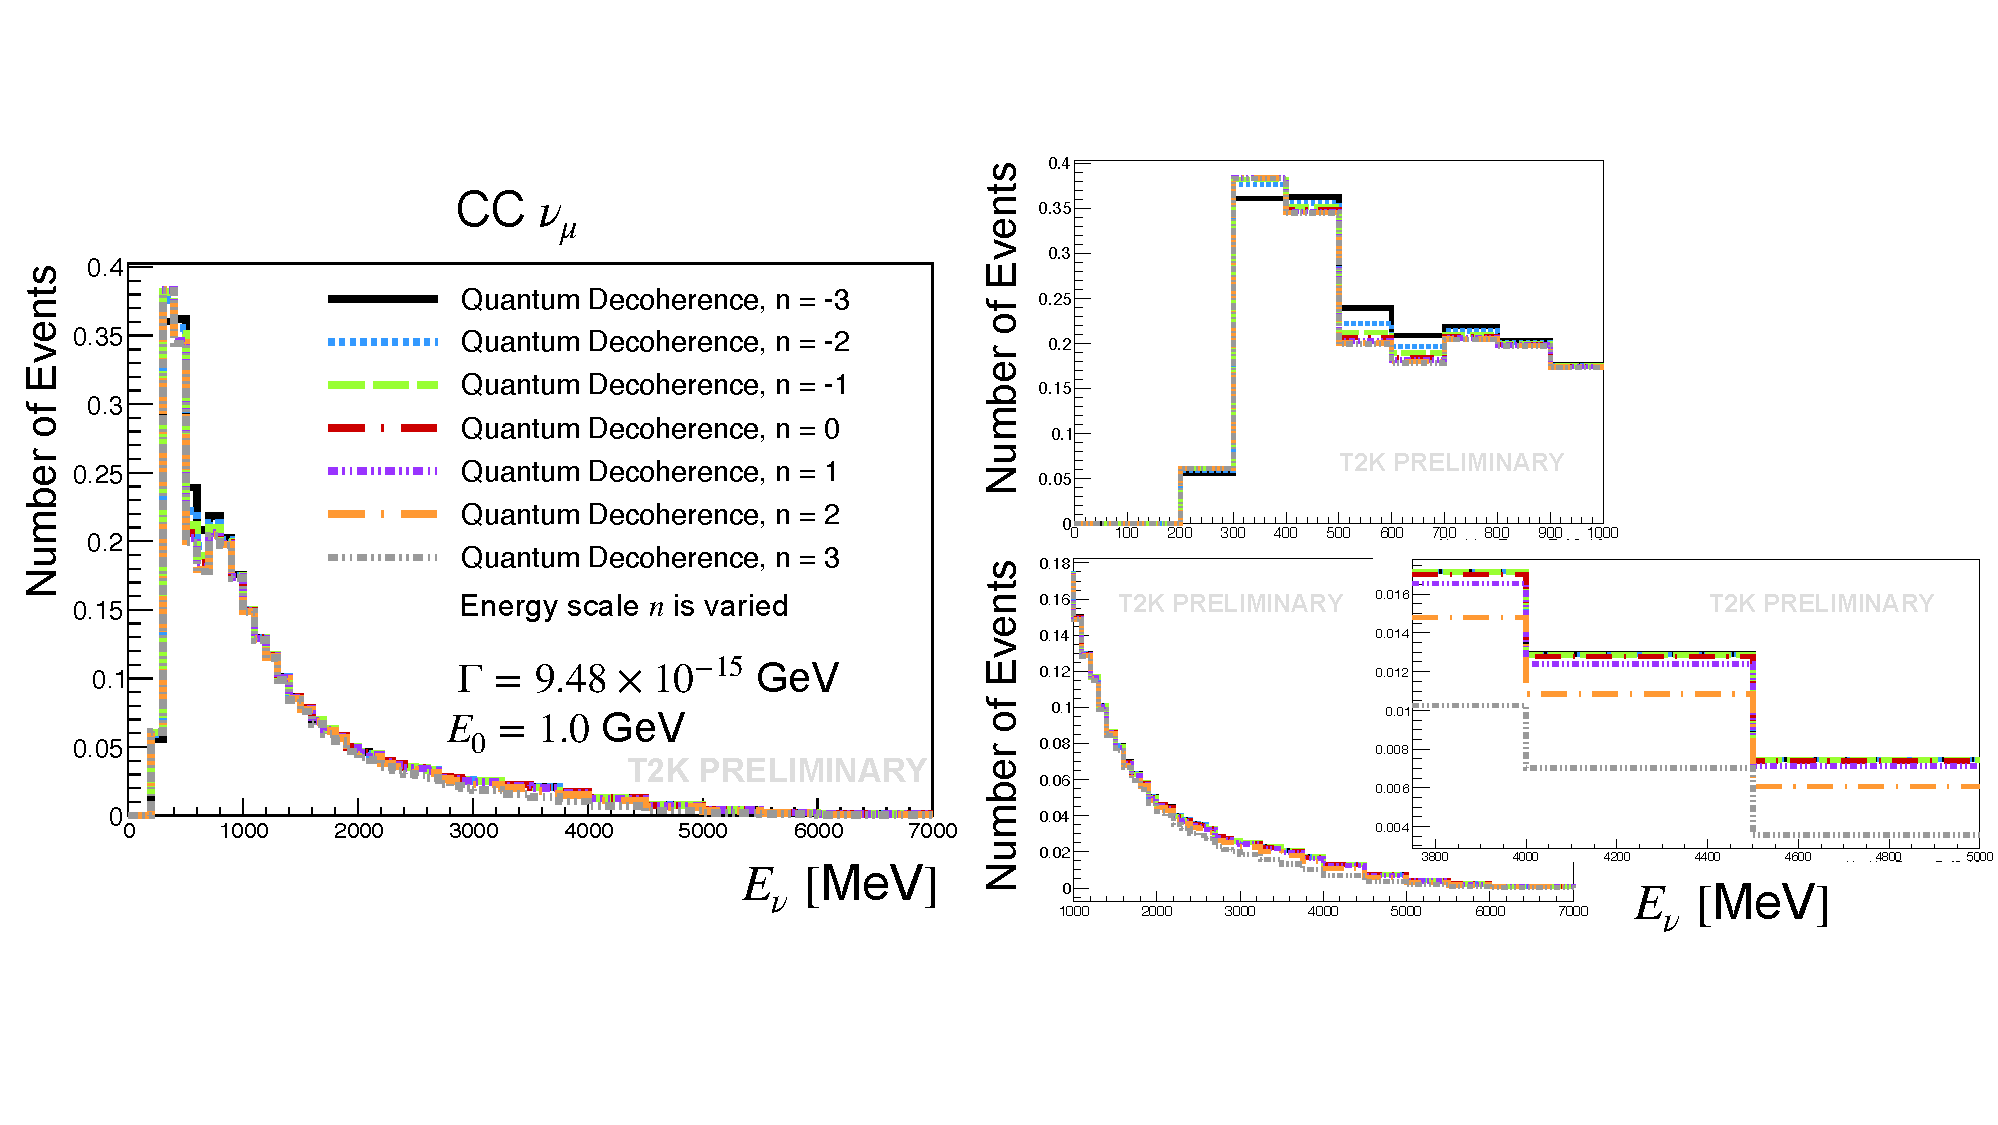
\includegraphics[width=1.\textwidth]
    {figures/QD_T2K_n_varied2.pdf}%{figures/QD_T2K_n_varied.pdf}
	\caption{Left: \acrshort{cc} muon-neutrino event rate and ratios. Right: Inlets of the event rate on the left for the lower (top) and higher (bottom) energy regions in \acrshort{t2k}. The energy scale exponent $n$ is varied while the decoherence strength is fixed at $\Gamma(E_0) = 9.48\times10^{-18}$ GeV.}
	\label{fig:qd_t2k_n_varied}
    \end{figure}
%

\begin{tabular}{|c|c|}
\hline
\rule[-1.2ex]{0pt}{3.5ex} $n$ & $\Gamma_{90\%}\ [\mathrm{eV}]$ \\
\hline
0 & $1.17 \cdot 10^{-15}\ [\mathrm{eV}]$ \\
1 & ... \\
2 & ... \\
3 & ... \\
\hline
\end{tabular}


\begin{table}
\caption[IceCube Quantum Decoherence Measurement (State Selection Model)]{IceCube Quantum Decoherence Measurement. The $90\%$ CL upper limits on the decoherence strength $\Gamma$ for each $n$ in $E_0=1\ \mathrm{GeV}$ in the State Selection Model.}
\renewcommand{\arraystretch}{1.2}
\begin{tabular}{|c|c|}
\hline
$n$ & $\Gamma^{90\%}\ [\mathrm{eV}]$ \\
\hline
0 & $1.17 \cdot 10^{-15}\ [\mathrm{eV}]$ \\
1 & $6.67 \cdot 10^{-19}\ [\mathrm{eV}]$ \\
2 & $9.48 \cdot 10^{-24}\ [\mathrm{eV}]$ \\
3 & $1.77 \cdot 10^{-28}\ [\mathrm{eV}]$ \\
\hline
\end{tabular}
\end{table}

\begin{table}
\caption[IceCube Quantum Decoherence Measurement (Phase Perturbation Model)]{IceCube Quantum Decoherence Measurement. The $90\%$ CL upper limits on the decoherence strength $\Gamma$ for each $n$ in $E_0=1\ \mathrm{GeV}$ in the Phase Perturbation Model.}
\renewcommand{\arraystretch}{1.2}
\begin{tabular}{|c|c|}
\hline
$n$ & $\Gamma^{90\%}\ [\mathrm{eV}]$ \\
\hline
0 & $1.18 \cdot 10^{-15}\ [\mathrm{eV}]$ \\
1 & $6.89 \cdot 10^{-19}\ [\mathrm{eV}]$ \\
2 & $9.80 \cdot 10^{-24}\ [\mathrm{eV}]$ \\
3 & $1.58 \cdot 10^{-28}\ [\mathrm{eV}]$ \\
\hline
\end{tabular}
\end{table}

\begin{table}
\caption[KM3NeT/ORCA Quantum Decoherence Measurement (Phase Perturbation Model)]{KM3NeT/ORCA Quantum Decoherence Measurement. The $90\%$ CL upper limits on the decoherence strength $\Gamma$ for each $n$ in $E_0=1\ \mathrm{GeV}$ in the Phase Perturbation Model.}
\renewcommand{\arraystretch}{1.2}
\begin{tabular}{|c|c|c|}
\hline
$n$ & $\Gamma^{90\%}_{21}\ [\mathrm{eV}]$ & $\Gamma^{90\%}_{31}\ [\mathrm{eV}]$ \\
\hline
-1 & $1.9 \cdot 10^{-13}\ [\mathrm{eV}]$ & $2.7 \cdot 10^{-13}\ [\mathrm{eV}]$ \\
-2 & $4.6 \cdot 10^{-12}\ [\mathrm{eV}]$ & $8.4 \cdot 10^{-12}\ [\mathrm{eV}]$ \\
\hline
\end{tabular}
\end{table}